\documentclass[English, Lau, oneside]{sapthesis}
%\usepackage{hyperref}
\usepackage{microtype}
\usepackage[english]{babel}
\usepackage[utf8]{inputenx}
\usepackage{graphicx}
\usepackage{float} % Include the float package
\usepackage{skmath}
\usepackage{amsmath, xparse}
\usepackage{wrapfig}
\usepackage{float}
\usepackage{amsmath,amssymb}
\usepackage{sidecap}
\usepackage{xcolor}
\usepackage{gensymb}
\usepackage{caption}
\usepackage{tabularx}
\usepackage{geometry}
\usepackage[utf8]{inputenx}
\usepackage{indentfirst}
\usepackage{microtype}
\usepackage[italian]{babel}
\usepackage{siunitx}
\DeclareMathOperator\erf{erf}
\usepackage{hyperref}
\usepackage{csvsimple}
\usepackage{subfig}
\usepackage{placeins}
\usepackage{subcaption}
\usepackage{xfrac}
\usepackage[makeroom]{cancel}
\usepackage{verbatim}
\usepackage{ gensymb }
\usepackage{ longtable }
\usepackage{geometry}
\usepackage{eucal}
%\usepackage{hyperref}
\usepackage{braket}
\usepackage{bbold}
\usepackage[hidelinks]{hyperref}
\usepackage{indentfirst}
\usepackage{microtype}
\usepackage{amsmath}
\usepackage{siunitx}
\usepackage{hyperref}

\usepackage[titles]{tocloft}


%\usepackage{chemformula}
%\usepackage{setspace}
%\usepackage{yfonts,color}
%\usepackage{siunitx}
%\usepackage{comment}
%\usepackage{multirow}
%\usepackage{varioref}
%\usepackage[bottom]{footmisc}
%\usepackage{wrapfig}
%\usepackage{float}
%\usepackage{type1cm}
%\usepackage{chngcntr}
%\onehalfspacing
%\counterwithout{footnote}{chapter}
\usepackage{hyperref}
\usepackage{hyperref}
\hypersetup{
			hyperfootnotes=true,			
			bookmarks=true,			
			colorlinks=true,
			linkcolor=red,
                        linktoc=page,
			anchorcolor=black,
			citecolor=red,
			urlcolor=blue,
			pdftitle={La natura particellare della materia oscura},
			pdfauthor={Enrico Bignozzi},
			pdfkeywords={thesis, sapienza, roma, university}
 }


\hypersetup{pdftitle={Sapthesis class example},pdfauthor={Francesco Beccari}}

% Remove in a normal thesis
\usepackage{lipsum}
\usepackage{curve2e}
\definecolor{gray}{gray}{0.4}
\newcommand{\bs}{\textbackslash}

% Commands for the titlepage
\title{Protein response in equilibrium and out of equilibrium conditions}
\author{Bignozzi Enrico}
\IDnumber{1855163}
\course{Corso di Laurea Magistrale in Fisica}
\courseorganizer{Facoltà di Scienze Matematiche, Fisiche e Naturali}
\AcademicYear{2025}
\copyyear{}
\advisor{Fabio Cecconi}
\coadvisor{}
\authoremail{bignozzi.1855163@studenti.uniroma1.it}

%\examdate{16 April 2013}
%\examiner{Prof. Nome Cognome}
%\examiner{Prof. Nome Cognome}
%\examiner{Dr. Nome Cognome}
%\versiondate{\today}
\begin{document}
\maketitle

\addcontentsline{toc}{chapter}{Indice}
\tableofcontents

%\begin{abstract}

%\end{abstract}

%\begin{acknowledgments}
    
%\end{acknowledgments}

\dedication{}

\newpage
\null
\thispagestyle{empty}
\newpage


% Do not use the starred version of the chapter command!


\newpage
\null
\thispagestyle{empty}
\newpage



\chapter*{Introduction}
\addcontentsline{toc}{chapter}{Introduction}
\noindent
Proteins are essential components of life and key to the functionality of living organisms. \cite{ref} \\
They are composed of a sequence of amino acids, a chain of amino acids, that fold into a three-dimensional structure that determines their function. 
The study of proteins is crucial for understanding the molecular basis of life and for the development of new drugs.\\
The determination of the three-dimensional structure of a protein is a fundamental step in the study of its function.
Among the main functions of proteins are:\cite{ref}
\begin{itemize}
    \item \textbf{Enzymatic catalysis}: Enzymatic proteins accelerate chemical reactions by reducing activation energy and regulating cellular metabolic processes.
    \item \textbf{Structural roles}: Some proteins, such as collagen or keratin, provide mechanical support and structural integrity to tissues.
    \item \textbf{Transport}: Molecules like hemoglobin facilitate oxygen transport, while other proteins transport nutrients and ions across cellular membranes.
    \item \textbf{Regulation and signaling}: Proteins play key roles in cellular signal transduction and the regulation of gene expression.
\end{itemize}
Our goal is to study the interactions between the amino acids that compose the protein, 
in order to understand how they fold into a functional structure.

\newpage
\section{Structure of amino acids}
\noindent Each amino acid consists of a central carbon atom (\(\alpha\)-carbon) bonded to four groups:\cite{ref2} \\
\begin{itemize}
    \item \textbf{Amino Group (\(-NH_2\))}: A basic functional group.
    \item \textbf{Carboxyl Group (\(-COOH\))}: An acidic functional group.
    \item \textbf{Side Chain (\(R\)-Group)}: This varies for each amino acid, giving it unique properties.
    \item \textbf{Hydrogen Atom}: A single hydrogen atom completes the structure.
\end{itemize}

The \(R\)-group, or side chain, determines the chemical properties of the amino acid, such as whether it is hydrophilic, hydrophobic, acidic, or basic.
\begin{figure}[H]
    \centering
    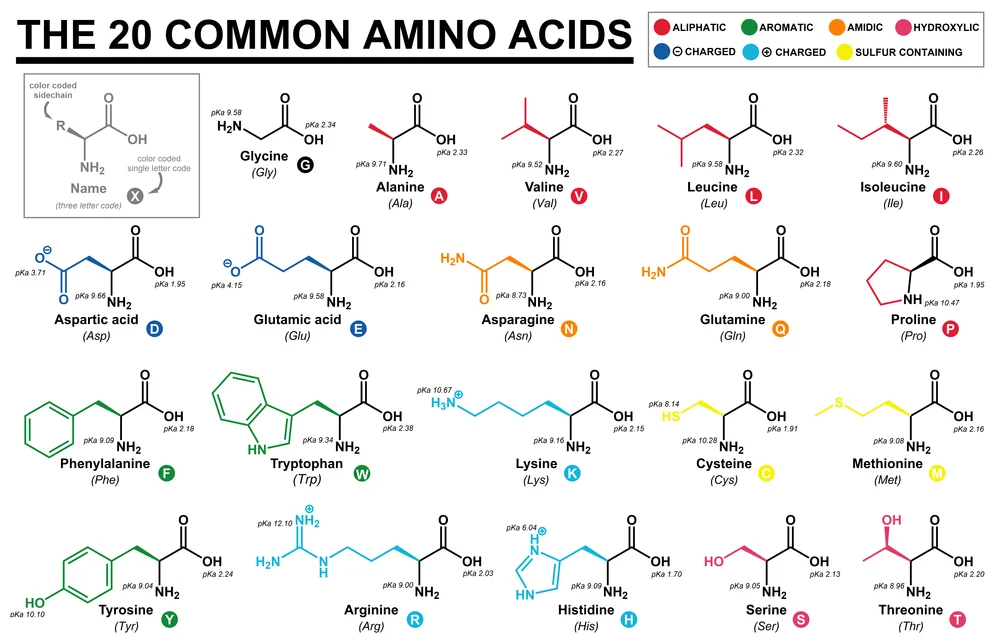
\includegraphics[width=1\textwidth]{/Users/enrico/PROTEINS/tesi/immagini_tesi_ingelse/ammino.png}
    \caption{Amino Acids}
\end{figure}
\newpage
\section{Protein structure}
\noindent The scructure of the protein is important because it determines its function. 
The structure of a protein is divided into four levels:\cite{ref4}
\subsection{Primary structure}
\noindent The primary structure refers to the linear sequence of amino acids in a protein chain, held together by peptide bonds. This sequence is unique for each protein and dictates the higher levels of structure.

\subsection{Secondary structure}
\noindent The secondary structure refers to the local folding of the protein chain into regular patterns such as alpha-helices and beta-pleated sheets. These structures are stabilized by hydrogen bonds between the backbone atoms of the amino acids.

\subsection{Tertiary structure}
\noindent The tertiary structure describes the three-dimensional folding of the entire protein molecule, including all its side chains. This level of structure is stabilized by interactions such as hydrogen bonds, ionic bonds, hydrophobic interactions, and disulfide bridges.

\subsection{Quaternary structure}
\noindent The quaternary structure applies to proteins that consist of more than one polypeptide chain. It describes how these chains are arranged and interact with each other to form the functional protein complex.
\begin{figure}[H]
    \centering
    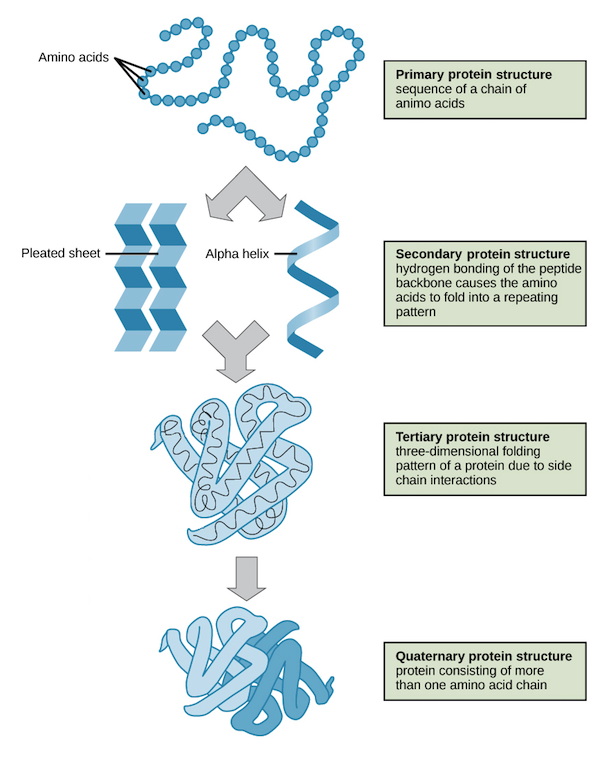
\includegraphics[width=0.5\textwidth]{/Users/enrico/PROTEINS/tesi/immagini_tesi_ingelse/71225d815cafcc09102504abdf4e10927283be98.png}
    \caption{Structures}
\end{figure}

This structure are due to the interactions between the amino acids that compose the protein. 
Following we will see our model for the interaction between the amino acids.
\newpage
\section{Allostericity}
\noindent Allostericity, from the Greek \textit{allos} (other) and \textit{stereos} (structure), is the phenomenon of the change of the protein structure by the trasmission of a signal from one site to another.\cite{ref5}
It refers to a phenomenon in which the interaction of a molecule (effector) with a specific site of a protein, known as the allosteric site, induces a conformational change that influences the functional activity of another site, usually the active site. 
This avoid the protein to do various tasks in a regulated way.
Additionally allostericity does not occur through direct interactions between the two sites but rather via changes in the network of intramolecular interactions that regulate the structure and dynamics of the protein.\\
From a thermodynamic perspective, allostericity can be described as a modulation of the distribution of a protein's energy microstates. 
In other words, the interaction with an allosteric effector alters the set of available conformational states, facilitating or inhibiting access to functional configurations.\cite{ref6}

Mathematically, the phenomenon can be represented as a variation in the population of microstates \(\{s_i\}\), described by a weighted Boltzmann distribution:\cite{ref6}

\[
P(s_i) = \frac{e^{-\Delta F(s_i)/k_BT}}{\sum_j e^{-\Delta F(s_j)/k_BT}}
\]

where \(\Delta F(s_i)\) represents the free energy associated with microstate \(s_i\), \(k_B\) is the Boltzmann constant, and \(T\) is the absolute temperature.

The allosteric effect can also be quantified by considering the change in free energy associated with the effector interaction. For a protein with two principal states, \(R\) (relaxed) and \(T\) (tense), the allosteric equilibrium can be expressed in terms of an equilibrium constant:\cite{ref6}

\[
L = \frac{[T]}{[R]}
\]
where \([T]\) and \([R]\) represent the relative concentrations of the two conformational states, where the presence of an effector modifies \(L\), stabilizing one state over the other.
Therefore proteins are not rigid structures; instead, they are ensembles of conformational states that fluctuate over temporal and spatial scales.

 So allosteric effectors,  can be represented as a perturbation that modifies the energy landscape of the conformational states \(\{E_i\}\), remodeling energy pathways and altering the probability \(P_i\) of each state, where:\cite{ref6}

\[
P_i = \frac{e^{-\beta E_i}}{Z}, \quad \text{with } Z = \sum_i e^{-\beta E_i}.
\]

\begin{figure}[h]
    \centering
    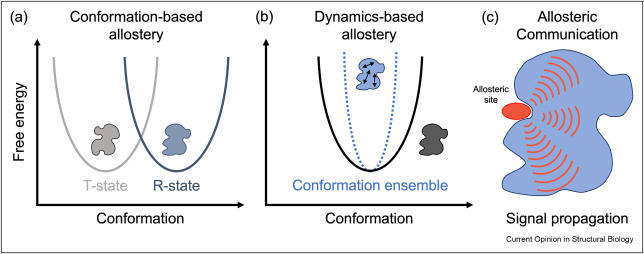
\includegraphics[width=\textwidth]{/Users/enrico/PROTEINS/tesi/immagini_tesi_ingelse/1-s2.0-S0959440X23002117-gr1.jpg}
    \caption{Schematic representation of allostericity: the interaction with an allosteric effector (site A) induces a conformational change that affects a distant site (site B).}
    \label{fig:allostericity_dynamics}
\end{figure}

This dynamic view integrates well with computational approaches such as molecular dynamics and interaction residue networks, which allow for the identification of specific pathways through which allosteric information propagates within the protein.


Understanding how and why the proteins fold into a functional structure it is useful for the study of the molecular basis of life and for the development of new drugs.
To study it we need to understand the causal mechanism and the propagation of the signal between the amino acids that compose the protein.
\newpage
\subsection{QUESTA PARTE LA METTO? LA SUA FINALITA E' FARE CAPIRE IN PRATICA AL LETTORE COSI' CHE SIA MENO ASTRATTA QUESTA PRIMA PARTE, DIMMI TU FABIO}
\subsection{Practical exemple of the mechanism of allostericity}
\noindent Hemoglobin, the oxygen-transporting protein within red blood cells, is a classic example of an allosteric protein.  \\
Its function is to bind oxygen in the lungs and release it efficiently in tissues where oxygen is needed. This process is regulated by its allosteric properties, which involve conformational changes and cooperative binding.

Hemoglobin exists in two main states:\cite{ref7}
\begin{itemize}
    \item \textbf{T-state (Tense):} This state has a lower affinity for oxygen and is stabilized in tissues where oxygen levels are low.
    \item \textbf{R-state (Relaxed):} This state has a higher affinity for oxygen and is stabilized in the oxygen-rich environment of the lungs.
\end{itemize}

When the first oxygen molecule binds to one of hemoglobin's four subunits, it induces a conformational change that increases the affinity of the remaining subunits for oxygen. 
This phenomenon is called \textit{cooperative binding} and is a hallmark of allosteric regulation.

Similarly, the release of oxygen in tissues is facilitated by other effectors, such as:
\begin{itemize}
    \item \textbf{Carbon dioxide (\(CO_2\))} and \textbf{protons (\(H^+\))}, which stabilize the T-state (Bohr effect).
    \item \textbf{2,3-Bisphosphoglycerate (2,3-BPG)}, which reduces oxygen affinity to promote oxygen release in tissues.
\end{itemize}

\subsection{Applications of understanding protein function}

\noindent Exploring how proteins function in dynamic ways has numerous practical uses in areas like medicine, technology, and diagnostics:

\begin{itemize}
    \item \textbf{Improving health treatments:}  
    Discovering new ways to interact with specific protein sites can open doors to advanced therapies for various illnesses. For instance, it could help create medicines that manage oxygen levels in the body or develop drugs to target diseases like cancer or infections.

    \item \textbf{Designing synthetic proteins:}  
    Insights into protein behavior are used to create innovative molecules, such as artificial blood substitutes or enzymes tailored for specific industrial or medical needs.

    \item \textbf{Advancing disease detection:}  
    Certain protein characteristics make them valuable markers for identifying and tracking health conditions, from diabetes to tissue damage, offering more precise diagnostic tools.

    \item \textbf{Innovating drug development:}  
    Strategies that focus on unique protein features can enhance drug effectiveness while minimizing unintended effects, paving the way for more targeted treatments in areas like cancer and heart disease.

    \item \textbf{Enhancing oxygen delivery:}  
    Studying proteins involved in oxygen transport can lead to improved therapies for people with limited oxygen levels, whether due to medical conditions or high-performance demands.

    \item \textbf{Supporting agriculture and environment:}  
    Understanding proteins in plants and microorganisms can boost food production or aid environmental cleanup, such as by improving nutrient efficiency or reducing carbon emissions.
\end{itemize}
\newpage
\section{PDZ Domain}
\noindent 
In molecular biology, a \textbf{domain} is a specific region of a protein that can perform a structural or functional role independently from the rest of the protein.\cite{ref8} \\
Domains are essential because they serve as modular units that recur and combine to form complex proteins with distinct functions.\cite{ref8} \\
Proteins often consist of multiple domains arranged in various combinations, creating multifunctional macromolecules capable of complex interactions. This domain architecture is essential for processes such as cell signaling, immune response, and metabolic regulation.\\
Moreover domains are not just structural units; they are also functional hubs that dictate the interactions and roles of proteins in cellular environments. \cite{ref8}

\subsection*{Definition of Domain}
\noindent A protein domain is generally defined by three key characteristics:\cite{ref8}
\begin{enumerate}
    \item \textbf{A structurally independent unit}: It is a portion of the protein that can fold into a stable three-dimensional structure on its own. This stability ensures that the domain can function even if other parts of the protein are absent or denatured. \\
    The ability of domains to independently fold is crucial for their versatility and functionality.
    \item \textbf{A functionally independent unit}: It can perform specific tasks, such as binding to a molecule or interacting with other proteins. For instance, the SH2 domain recognizes phosphorylated tyrosine residues, enabling signal transduction pathways.\\
    Some domains exhibit functional independence.
    \item \textbf{An evolutionary modular unit}: Domains are often reused in different proteins during evolution, allowing for the development of new functions. This modularity is evident in protein families where similar domains are observed across diverse organisms, reflecting a shared evolutionary origin. 
\end{enumerate}

Domains are classified based on their structure, sequence, or function, with databases such as Pfam and SMART cataloging thousands of examples.\cite{pfam} These resources are invaluable for researchers aiming to predict protein function, identify evolutionary relationships, and design novel biomolecules with tailored functionalities. Structural studies and computational analyses continue to expand our understanding of domain architectures, revealing the intricate interplay between form and function in proteins.

\subsection*{The PDZ Domain}
\noindent The \textbf{PDZ domain} is a well-studied example of a protein domain. It is named after the three proteins in which it was first identified:\cite{ref8}
\begin{itemize}
    \item \textbf{P}SD-95 (Postsynaptic density protein 95),
    \item \textbf{D}lgA (Drosophila discs large protein),
    \item \textbf{Z}O-1 (Zona Occludens 1).
\end{itemize}
The PDZ domain exemplifies the modularity of protein domains, as it appears in a wide variety of proteins across eukaryotes, highlighting its evolutionary significance. PDZ domains organize and stabilize large multiprotein complexes. This prevalence underscores their critical role in maintaining cellular architecture and facilitating biochemical signaling pathways.
\subsubsection*{Characteristics of the PDZ Domain}
\begin{itemize}
    \item \textbf{Length}: Typically consists of 80--90 amino acids, making it a compact and efficient structural module. Despite its small size, the PDZ domain has remarkable functional versatility, binding to a diverse array of target peptides with high specificity.
    \item \textbf{Main Function}: Facilitates protein-protein interactions by recognizing specific peptide sequences, often located at the C-terminal region of target proteins. This ability to bind peptides with high specificity and affinity makes PDZ domains essential for organizing protein complexes. Such specificity arises from the conserved binding groove, which accommodates peptide motifs in a lock-and-key fashion.\cite{song1997}
    \item \textbf{Biological Role}:
    \begin{itemize}
        \item Assembling protein complexes at cellular membranes. For instance, PDZ domains play a pivotal role in assembling synaptic proteins, ensuring efficient signal transduction in neurons.
        \item Cellular signaling, particularly in pathways regulating cell growth and differentiation. PDZ-mediated interactions are involved in key signaling cascades, including those controlled by receptor tyrosine kinases and G-protein-coupled receptors.
    \end{itemize}
    \item \textbf{Structure}: The PDZ domain has a characteristic structure composed of an antiparallel beta-sheet and two alpha-helices. This conserved fold forms a groove that interacts with the target peptide, contributing to its specificity. The structural plasticity of PDZ domains allows them to adapt to various ligands, enhancing their functional diversity.\cite{harris2001}
\end{itemize}

\subsection*{The PDZ Domain in the 3LNX Protein}

\noindent The 3LNX protein, on which we will work, provides a clear example of how a PDZ domain binds to a target peptide. This structure offers important insights into the functioning of these domains:

\begin{enumerate}
    \item \textbf{How the peptide binds:}
    
    In the 3LNX protein, the PDZ domain has a "hydrophobic pocket" that accommodates the peptide it binds to. This binding is very precise and stable, thanks to connections such as hydrogen bonds and weak interactions between nearby molecules. Small changes in the sequence of the peptide can influence how well the PDZ domain binds.

    \item \textbf{Domain flexibility:}
    
    When the peptide binds, the PDZ domain slightly adjusts its shape. This shows that it is very flexible and capable of interacting with many different types of molecules. This flexibility is essential for its role in cellular communication.

    \item \textbf{Biological importance:}
    
    PDZ domains, like the one in the 3LNX protein, are fundamental in synapse organization, where they help assemble signaling complexes necessary for brain function. Knowledge of this protein has been used to design molecules that can regulate these interactions, with potential applications for treating diseases.
\end{enumerate}







\chapter{Modeling the Interaction between Amino Acids: GNM}
\noindent The interactions between the amino acids that compose the protein are crucial for the folding of the protein into a functional structure.  
Thus, we need a Hamiltonian to describe the system. 

If the protein is at equilibrium, we expect that the Hamiltonian is a function of a potential that depends on the position of every atom constituting the PDZ-specific domain.  
Therefore, my Hamiltonian \( H \) can be written as \( H = V(\mathbf{r}) \), where \( \mathbf{r} \) is the vector containing the positions of every atom that constitutes the protein.  

Since this is a very complex system, we cannot solve the problem exactly, so we must use an approximation. The second-order approximation of a function \( V(\mathbf{r}) \), around an equilibrium point \( \mathbf{r}_0 \), can be expressed as:\cite{ref9}

\begin{equation}
V(\mathbf{r}) \approx V(\mathbf{r}_0) + \nabla V(\mathbf{r}_0)^\top (\mathbf{r} - \mathbf{r}_0) + \frac{1}{2} (\mathbf{r} - \mathbf{r}_0)^\top \mathbf{H_V} (\mathbf{r} - \mathbf{r}_0),\label{hessian}
\end{equation}

where:
\begin{itemize}
    \item \( V(\mathbf{r}_0) \) is the value of the function at the equilibrium point \( \mathbf{r}_0 \).
    \item \( \nabla V(\mathbf{r}_0) \) is the gradient of the function, defined as:
    \begin{equation}
    \nabla V(\mathbf{r}) = \frac{\partial V}{\partial \mathbf{r}} \bigg|_{\mathbf{r} = \mathbf{r}_0},
    \end{equation}
    which equals zero if \( \mathbf{r}_0 \) represents a minimum point, corresponding to the equilibrium position.
    \item \( \mathbf{H_V} \) is the \textbf{Hessian matrix} of \( V(\mathbf{r}) \), defined as:
    \begin{equation}
    \mathbf{H_V} = \frac{\partial^2 V}{\partial \mathbf{r}^2} \bigg|_{\mathbf{r} = \mathbf{r}_0},
    \end{equation}
    \[
    \mathbf{H} = \begin{bmatrix}
    \frac{\partial^2 V}{\partial x_1^2} & \frac{\partial^2 V}{\partial x_1 \partial x_2} & \cdots & \frac{\partial^2 V}{\partial x_1 \partial x_{3N}} \\
    \frac{\partial^2 V}{\partial x_2 \partial x_1} & \frac{\partial^2 V}{\partial x_2^2} & \cdots & \frac{\partial^2 V}{\partial x_2 \partial x_{3N}} \\
    \vdots & \vdots & \ddots & \vdots \\
    \frac{\partial^2 V}{\partial x_{3N} \partial x_1} & \frac{\partial^2 V}{\partial x_{3N} \partial x_2} & \cdots & \frac{\partial^2 V}{\partial x_{3N}^2}
    \end{bmatrix}.
    \]
    It is a symmetric matrix that describes the curvature of \( V(\mathbf{r}) \) around \( \mathbf{r}_0 \).
\end{itemize}

It is important to note that the \textbf{Hessian matrix} \( \mathbf{H_V} \) should not be confused with the \textbf{Hamiltonian}, which represents the total energy of a system in terms of conjugate coordinates (positions and momenta).  

Thus, apart from constants, the Hamiltonian can be approximated as:

\begin{equation}
V(\mathbf{r}) \approx \frac{1}{2} (\mathbf{r} - \mathbf{r}_0)^\top \mathbf{H_V} (\mathbf{r} - \mathbf{r}_0). \label{1.1}
\end{equation}
This modeling is called Gaussian Network Model (GNM) and is comminly used to study the dynamics of proteins.\\
To reduce the computational complexity of the problem while preserving essential structural features, we focus solely on the \(\alpha\)-carbon atoms because:

\begin{itemize}
    \item \(\alpha\)-carbon atoms form the backbone of the protein, defining its overall structure and shape.
    \item Their positions are sufficient to reconstruct the global three-dimensional conformation of the protein.
    \item Focusing on \(\alpha\)-carbons significantly reduces the complexity of the system, lowering the number of degrees of freedom and making calculations more efficient.
    \item The dynamics of \(\alpha\)-carbons often capture the collective motions of the protein, crucial for understanding its function (e.g., domain movements, opening of active sites).
    \item Experimental techniques such as X-ray crystallography and NMR frequently provide high-resolution data specifically for \(\alpha\)-carbon atoms, serving as reference points for modeling.
\end{itemize}

This model is overall extendable to all other atoms of the protein.
\newpage

\section{Interpretation of the Taylor Expansion}
\noindent  Equation \eqref{1.1} can be interpreted not only as the Hamiltonian of the harmonic oscillator (spring-system) but also as a network model, where every \(\alpha\)-carbon atom is a node interacting with other nodes.\cite{ref9}

\subsubsection{Definition of a Graph}
\noindent A graph \( G \) is a mathematical structure used to model pairwise relations between objects. It consists of a set of vertices \( V \) (also called nodes) and a set of edges \( E \), where each edge connects a pair of vertices.\cite{ref11}\\
Graphs can be directed or undirected, weighted or unweighted, depending on the nature of the relationships they represent.

\begin{figure}[h]
    \centering
    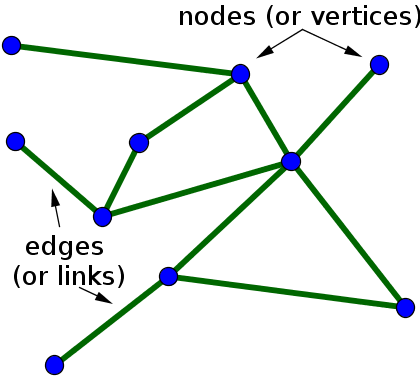
\includegraphics[width=\textwidth]{/Users/enrico/PROTEINS/tesi/immagini_tesi_ingelse/small_undirected_network_labeled-2.png}    
    \caption{Schematic representation of a Network.}
    \label{fig:Network}
\end{figure}

\subsubsection{Kirchhoff Matrix (Laplacian Matrix)}
\noindent The Kirchhoff matrix, also known as the graph Laplacian, is a matrix representation of a graph that encodes information about its structure. For a graph \( G \) with \( n \) vertices, the Laplacian matrix \( L \) is defined as:\cite{ref11}

\begin{equation}
    L = D - A \label{Kirchhoff}
\end{equation}
Here:
- \( D \) is the degree matrix, a diagonal matrix defined as:
\begin{equation}
    D_{ij} = 
    \begin{cases} 
      \deg(v_i) & \text{if } i = j, \\
      0 & \text{if } i \neq j,
    \end{cases}
\end{equation}
where \( \deg(v_i) \) is the degree of vertex \( v_i \), i.e., the number of edges connected to vertex \( i \).

- \( A \) is the adjacency matrix, a square matrix defined as:
\begin{equation}
    A_{ij} = 
    \begin{cases} 
      1 & \text{if there is an edge between vertices } v_i \text{ and } v_j, \\
      0 & \text{otherwise}.
    \end{cases}
\end{equation}

The Laplacian matrix \( L \), derived from \( D \) and \( A \), captures essential properties of the graph, such as connectivity and flow. It is widely used in spectral graph theory, network analysis, and machine learning.
\subsubsection{Properties of the Degree Matrix}
The degree matrix \( D \) has the following properties:\cite{ref11}
\begin{itemize}
    \item \textbf{Diagonal Matrix:} \( D \) is diagonal, meaning all off-diagonal elements are zero.
    \item \textbf{Non-Negative Entries:} Each diagonal element \( d_{ii} \) represents the degree of vertex \( i \), which is always non-negative.
    \item \textbf{Relation to Graph Order:} For simple graphs, the sum of all diagonal elements of \( D \) equals twice the number of edges, i.e., \( \mathrm{trace}(D) = 2|E| \).
\end{itemize}

\subsubsection{Properties of the Adjacency Matrix}
\noindent The adjacency matrix \( A \) encodes the edge structure of the graph and has the following properties:\cite{ref11}
\begin{itemize}
    \item \textbf{Symmetry:} For undirected graphs, \( A \) is symmetric, i.e., \( a_{ij} = a_{ji} \).
    \item \textbf{Binary Entries:} For unweighted graphs, each element \( a_{ij} \in \{0, 1\} \), where \( 1 \) indicates the presence of an edge between \( i \) and \( j \), and \( 0 \) indicates absence.
    \item \textbf{Weighted Graphs:} For weighted graphs, \( a_{ij} \) takes the weight of the edge between vertices \( i \) and \( j \).
    \item \textbf{Self-Loops:} Diagonal entries \( a_{ii} \) indicate self-loops. For simple graphs, \( a_{ii} = 0 \).
    \item \textbf{Spectral Properties:} The eigenvalues of \( A \) provide insights into graph connectivity and other structural properties, such as bipartiteness and clustering.
\end{itemize}
\subsubsection{Mathematical Properties of the Network}
\noindent The graph Laplacian has several important mathematical properties:\cite{ref11}
\begin{itemize}
    \item \textbf{Symmetry:} For undirected graphs, \( L \) is symmetric and thus diagonalizable.
    \item \textbf{Positive Semi-definiteness:} The Laplacian matrix \( L \) is positive semi-definite, meaning that all its eigenvalues are non-negative.
    \item \textbf{Eigenvalues:} The smallest eigenvalue of \( L \) is always \( 0 \), corresponding to the eigenvector \( \mathbf{1} \) (a vector of all ones). The multiplicity of the zero eigenvalue indicates the number of connected components in the graph.
    \item \textbf{Combinatorial Interpretation:} The determinant of the reduced Laplacian matrix (obtained by removing one row and one column) gives the number of spanning trees in the graph.
\end{itemize}

\subsubsection{Inverse of Weighted Laplacian (Pseudo-Inverse)}
For a connected graph, the weighted Laplacian \( L \) is not invertible due to the zero eigenvalue. However, the Moore-Penrose pseudo-inverse \( L^+ \) can be computed. 

The pseudo-inverse is used in various applications such as electrical network analysis, random walks, and graph-based optimization.\\ It satisfies:

\[
L^+ L = L L^+ = I - \frac{1}{n} \mathbf{1} \mathbf{1}^\top
\]

where \( n \) is the number of nodes and \( \mathbf{1} \) is a vector of all ones.
So it is the inverse of L in the subspace where L is invertible and minimize this difference $I - \frac{1}{n} \mathbf{1} \mathbf{1}^\top$.
\newpage
\section{Gaussian Network Model (GNM) and characteristics}
\noindent The Hamiltonian of the system can be expressed, following \eqref{1.1}, as:\cite{ref12}
\begin{equation}
    H(\mathbf{r}) \approx \frac{1}{2} (\mathbf{r} - \mathbf{r}_0)^\top \mathbf{K} (\mathbf{r} - \mathbf{r}_0),
\end{equation}
where \( \mathbf{K} \) is the Laplacian matrix. For simplicity, we can rewrite it as:
\begin{equation}
    H(\mathbf{r}) \approx \frac{1}{2} \mathbf{r}^\top \mathbf{K} \mathbf{r},
\end{equation}
or, in components:
\begin{equation}
    H(\mathbf{r}) \approx \frac{1}{2} \sum_{i,j} r_i K_{ij} r_j.
\end{equation}
Here, \(\mathbf{r}\) represents the displacement vector of atoms from their equilibrium positions.\\
This formulation of the system leads to several important properties and characteristics.

Initially, the probability density at equilibrium is given by:\cite{ref12}
\begin{equation}
    P(\mathbf{r}) = \frac{1}{Z} e^{-\beta H(\mathbf{r})},
\end{equation}
where the partition function \(Z\) is:
\begin{equation}
    Z = \int e^{-\beta H(\mathbf{r})} \, d\mathbf{r}.
\end{equation}

\subsubsection{Mean Position}
\noindent The mean position \(\langle \mathbf{r} \rangle\) can be calculated as:\cite{ref12}
\begin{equation}
    \langle \mathbf{r} \rangle = \int \mathbf{r} P(\mathbf{r}) \, d\mathbf{r},
\end{equation}
where:
\begin{equation}
    P(\mathbf{r}) = \frac{1}{Z} e^{-\frac{\beta}{2} \mathbf{r}^\top \mathbf{K} \mathbf{r}},
\end{equation}
and the partition function is:\cite{ref12}
\begin{equation}
    Z = \int e^{-\frac{\beta}{2} \mathbf{r}^\top \mathbf{K} \mathbf{r}} \, d\mathbf{r}.
\end{equation}

Substituting \(P(\mathbf{r})\) into the expression for \(\langle \mathbf{r} \rangle\), we obtain:
\begin{equation}
    \langle \mathbf{r} \rangle = \frac{1}{Z} \int \mathbf{r} e^{-\frac{\beta}{2} \mathbf{r}^\top \mathbf{K} \mathbf{r}} \, d\mathbf{r}.
\end{equation}

Since the integrand \(\mathbf{r} e^{-\frac{\beta}{2} \mathbf{r}^\top \mathbf{K} \mathbf{r}}\) is symmetric with respect to \(\mathbf{r}\), and there are no linear terms in the Hamiltonian, the Gaussian distribution is centered at \(\mathbf{r} = 0\). Therefore:\cite{ref12}
\begin{equation}
    \langle \mathbf{r} \rangle = 0.
\end{equation}

\subsubsection{Covariance}
\noindent The covariance between \(r_i\) and \(r_j\) is defined as:\cite{ref12}
\begin{equation}
    \text{Cov}(r_i, r_j) = \langle r_i r_j \rangle - \langle r_i \rangle \langle r_j \rangle.
\end{equation}

Since \(\langle r_i \rangle = 0\), it simplifies to:
\begin{equation}
    \text{Cov}(r_i, r_j) = \langle r_i r_j \rangle.
\end{equation}

Using the Boltzmann distribution:
\begin{equation}
    P(\mathbf{r}) = \frac{1}{Z} e^{-\frac{\beta}{2} \mathbf{r}^\top \mathbf{K} \mathbf{r}},
\end{equation}
we calculate:
\begin{equation}
    \langle r_i r_j \rangle = \frac{1}{Z} \int r_i r_j e^{-\frac{\beta}{2} \mathbf{r}^\top \mathbf{K} \mathbf{r}} \, d\mathbf{r}.
\end{equation}

For a Gaussian distribution, the covariance matrix is given by:
\begin{equation}
    \bm{\Sigma} = \beta^{-1} \mathbf{K}^{-1} = \langle r_i r_j \rangle,
\end{equation}
where \((\mathbf{K}^{-1})_{ij}\) represents the \((i,j)\)-th element of \(\mathbf{K}^{-1}\). Thus:
\begin{equation}
    \text{Cov}(r_i, r_j) = \frac{1}{\beta} (\mathbf{K}^{-1})_{ij}.
\end{equation}



\subsection*{QUESTA PARTE IN CUI METTO LA DERIVAZIOEN DEI BETA FACTORS LA METTO? Referenza materia condensata sapienza}
\subsection*{Derivation of diffraction intensity with atomic vibrations}
\noindent The diffraction intensity in crystallography is influenced by the atomic vibrations around their mean positions. These vibrations are characterized by the mean squared displacement, denoted as $\langle u^2 \rangle$. To derive the expression for intensity, we start with the electron density modulated by atomic displacement.

Let the position of an atom be $\mathbf{r}$, with its displacement modeled as a Gaussian distribution around its mean position $\mathbf{r_0}$. The thermal motion leads to a modification of the scattering factor:
\[
f(\mathbf{q}) = f_0(\mathbf{q}) \cdot e^{-2\pi i \mathbf{q} \cdot \mathbf{u}}
\]
where:
\begin{itemize}
    \item $f_0(\mathbf{q})$: scattering factor for a stationary atom,
    \item $\mathbf{q}$: scattering vector,
    \item $\mathbf{u}$: displacement from the mean position.
\end{itemize}

The observed intensity $I(\mathbf{q})$ is proportional to the squared magnitude of the structure factor $F(\mathbf{q})$:
\[
I(\mathbf{q}) \propto |F(\mathbf{q})|^2,
\]
where $F(\mathbf{q})$ is the sum over all atomic contributions:
\[
F(\mathbf{q}) = \sum_j f_j(\mathbf{q}) e^{2\pi i \mathbf{q} \cdot \mathbf{r}_j}.
\]

Now consider the thermal vibrations. Averaging over the Gaussian distribution of displacements yields a damping factor:
\[
\langle e^{-2\pi i \mathbf{q} \cdot \mathbf{u}} \rangle = e^{-2\pi^2 \langle (\mathbf{q} \cdot \mathbf{u})^2 \rangle}.
\]
Assuming isotropic vibrations, this simplifies to:
\[
\langle (\mathbf{q} \cdot \mathbf{u})^2 \rangle = |\mathbf{q}|^2 \langle u^2 \rangle,
\]
where $\langle u^2 \rangle$ is the mean squared displacement. Substituting this back, the intensity is:
\[
I(\mathbf{q}) \propto |F(\mathbf{q})|^2 e^{-8\pi^2 \langle u^2 \rangle |\mathbf{q}|^2}.
\]

The factor $B = 8\pi^2 \langle u^2 \rangle$ emerges naturally, leading to:
\[
I(\mathbf{q}) \propto |F(\mathbf{q})|^2 e^{-B |\mathbf{q}|^2}.
\]

\subsection*{Evaluation of beta factors and model quality}
\noindent In crystallography, the Beta factors (\(B\)) are an important metric to assess the quality of a structural model. The value of \(B\) is given by:
\begin{equation}
    B = 8\pi^2 \langle u^2 \rangle = 8\pi^2 \frac{k_B T}{k_{\text{eff}}} \label{Kirchhoff}
\end{equation}

Where:
\begin{itemize}
    \item \(\langle u^2 \rangle\): mean squared atomic displacement,
    \item \(k_B\): Boltzmann constant,
    \item \(T\): absolute temperature,
    \item \(k_{\text{eff}}\): effective spring constant (describing atomic rigidity).
\end{itemize}


\subsection*{Importance of the beta factor as a metric of model accuracy}
\noindent The beta factor ($B$) is a crucial metric in crystallographic modeling for several reasons:

\subsubsection*{1. Representation of atomic dynamics}
The beta factor reflects the thermal vibrations and dynamic behavior of atoms within the crystal. High $B$ values indicate greater atomic mobility or disorder, while low $B$ values suggest rigidity.

\subsubsection*{2. Assessment of structural flexibility}
Regions with elevated beta factors often correspond to flexible or disordered parts of the molecule, such as loops, termini, or unstructured regions. These provide insights into the functional dynamics of the macromolecule.

\subsubsection*{3. Indicator of model quality}
Unrealistically high or low beta factors across the structure can indicate modeling errors or issues with data quality, such as:
\begin{itemize}
    \item Poor resolution of the diffraction data.
    \item Incorrect assignment of atomic positions.
    \item Misrepresentation of isotropic vs. anisotropic motion.
\end{itemize}
\subsubsection*{4. Validation of refinement}
\noindent During model refinement, the beta factors are optimized to fit the experimental data. If the refinement process yields consistent and reasonable beta factors, it supports the accuracy of the atomic model.
\newpage


\section*{Model Evaluation: RMSE and MAE    {QUESTA IDEM NON SO SE METTERLA O NO. SCELGO IN FUNZIONE SE METTO QUESTE METRICHE DI ERRORE NELLA TESI DOPO}
}\label{sec:Evaluation}
\subsection*{RMSE: Root Mean Square Error}
\noindent The formula for RMSE is:
\[
\text{RMSE} = \sqrt{\frac{1}{n} \sum_{i=1}^n (y_i - \hat{y}_i)^2}
\]
Where:
\begin{itemize}
    \item \(y_i\): observed values,
    \item \(\hat{y}_i\): predicted values,
    \item \(n\): total number of data points.
\end{itemize}
\subsection*{MAE: Mean Absolute Error}
\noindent The formula for MAE is:
\[
\text{MAE} = \frac{1}{n} \sum_{i=1}^n |y_i - \hat{y}_i|
\]
Where:
\begin{itemize}
    \item \(y_i\): observed values,
    \item \(\hat{y}_i\): predicted values,
    \item \(n\): total number of data points.
\end{itemize}

\newpage
\chapter{Introduction to causality and causality in allosteric mechanisms of proteins (Qui è molto sottile il discorso e probabilmente non dovrei toccare alcuni punti)}

\noindent Correlation not only hinders testing the quality of models through beta factors but also obstructs understanding interactions and the relations between nodes/residues.\\
Our primary aim is to identify the allosteric site—the region from which a signal is transmitted to other sites of the protein, but as is often said, correlation does not imply causation.

\begin{figure}[h]
    \centering
    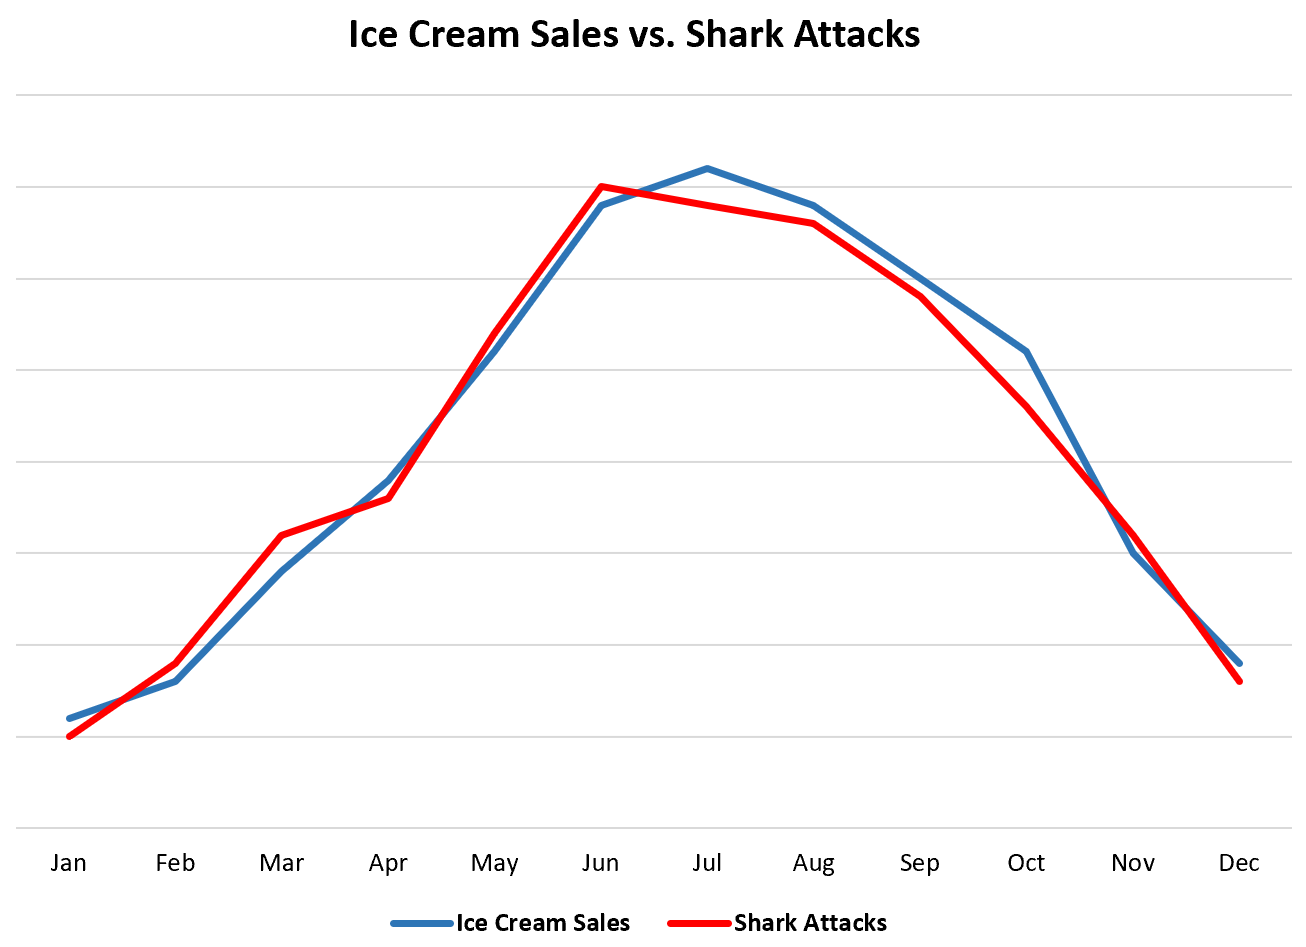
\includegraphics[width=\textwidth]{/Users/enrico/PROTEINS/tesi/immagini_tesi_ingelse/corrCause1.png}    
    \caption{Correlation is not causation.}
    \label{fig:Correlation is not causation}
\end{figure}

Causality refers to the relationship between causes and effects, where one event (the cause) directly influences or produces another event (the effect). 

Causality is a foundational concept across disciplines, including physics, philosophy, and statistics. It implies a directional influence, where the cause precedes the effect and is necessary, sufficient, or contributory for the effect to occur.

In mathematical terms, causal relationships are often modeled as:\cite{ref14}
\[
B = f(A, \text{other factors}),
\]
where \( f \) describes how \( A \) and other factors jointly determine \( B \). 

Experimentally, causality is typically established through controlled interventions and the observation of resulting changes.
\newpage
\section*{Deterministic and Stochastic Causality}

\noindent Causality can be classified into two main types: deterministic and stochastic.

\subsection*{Deterministic Causality}

\noindent Deterministic causality implies that a specific cause invariably leads to a specific effect. If an event \( A \) causes an event \( B \), then \( B \) always occurs whenever \( A \) occurs. This relationship can be expressed as \( A \implies B \), meaning \( A \) is both necessary and sufficient for \( B \). Deterministic causality is observed in systems governed by precise physical laws, such as classical mechanics, where given initial conditions and forces, trajectories are entirely predictable.

\subsection*{Stochastic Causality}

\noindent Stochastic causality acknowledges that many causal relationships are probabilistic rather than absolute. Here, the occurrence of \( A \) increases the likelihood of \( B \), but \( B \) does not always follow \( A \). This is expressed probabilistically as \( P(B|A) > P(B|\neg A) \), indicating that \( A \) raises the probability of \( B \). Stochastic causality is prevalent in complex systems like biology or social sciences, where multiple interacting factors and inherent randomness influence outcomes. For example, smoking increases the probability of lung cancer, though not all smokers develop the disease.

Both deterministic and stochastic causality are critical for understanding natural phenomena. Deterministic causality offers precise predictive power, while stochastic causality is indispensable for modeling systems where randomness and variability play significant roles. Together, they provide a comprehensive framework for analyzing causal relationships.
\newpage
\section*{Geometric Perspective of Causality and Shannon Entropy (questa è la parte piu' da togliere fra tutte probabilmente)}

\noindent When all dimensions or variables of a system are fully known, uncertainty about future states vanishes, transitioning the system into a deterministic regime. This idea relates to Shannon entropy, defined as:
\[
H(X) = -\sum_{i} P(x_i) \log P(x_i),
\]
where \( X \) is a random variable with possible states \( x_i \), and \( P(x_i) \) is the probability of \( x_i \). When \( P(x_i) = \delta(x_i) \) -> \( H(X) = 0 \), the system has no uncertainty, indicating complete predictability.
So if my target variable has the distirbution of the delta function, the entropy is zero, so the system is deterministic.
In deterministic systems, knowing all dimensions eliminates ambiguity, enabling precise predictions of future states. However, in practice i don't know all the dimensions of my system.
Thus, while \( H(X) = 0 \) theoretically implies determinism, real-world complexities and limitations must be accounted for.


To understand the causality of allosteric mechanisms in proteins, it is crucial to investigate the physical interactions and pathways that transmit signals between distant sites. For this reason, additional indicators are needed.
\newpage
\section*{Correlation}
\subsection{Correlation Between Fluctuations}
\noindent
The correlation between two variables, such as the fluctuations in the positions of particles \( i \) and \( j \), provides insight into how these components of the system interact.\\
The correlation function is defined as:\cite{ref13}
\begin{equation}
    C_{ij} = \langle \delta \mathbf{r}_i \cdot \delta \mathbf{r}_j \rangle, \label{correlation}
\end{equation}
where:
\begin{itemize}
    \item \( \delta \mathbf{r}_i = \mathbf{r}_i - \langle \mathbf{r}_i \rangle \) is the deviation of the position of particle \( i \) from its equilibrium value.
    \item \( \delta \mathbf{r}_j = \mathbf{r}_j - \langle \mathbf{r}_j \rangle \) is the deviation of the position of particle \( j \) from its equilibrium value.
    \item \( \langle \cdot \rangle \) denotes an ensemble average.
\end{itemize}

The correlation \( C_{ij} \) quantifies the degree to which the positions of particles \( i \) and \( j \) are linearly related at equilibrium.

\subsection*{Physical Interpretation of Correlations}

\noindent The correlation \( C_{ij} \) reflects how strongly two particles are connected in the system:
\begin{itemize}
    \item \textbf{Positive correlation:} A positive \( C_{ij} > 0 \) indicates that fluctuations in \( \mathbf{r}_i \) and \( \mathbf{r}_j \) tend to occur in the same direction, suggesting cooperative behavior or a direct connection.
    \item \textbf{Negative correlation:} A negative \( C_{ij} < 0 \) implies that fluctuations in \( \mathbf{r}_i \) and \( \mathbf{r}_j \) tend to occur in opposite directions, indicating opposing interactions or constraints between the particles.
    \item \textbf{Zero correlation:} A correlation of \( C_{ij} = 0 \) indicates no linear relationship between the fluctuations, suggesting either independence or non-linear interactions.
\end{itemize}

\subsection*{Why Correlation Alone is Not Causation}

\noindent While correlations reveal interactions, they do not establish a causal relationship. The limitations include:
\begin{itemize}
    \item \textbf{Symmetry:} Correlation is symmetric (\( C_{ij} = C_{ji} \)), whereas causality is asymmetric. The fact that \( i \) is correlated with \( j \) does not imply that \( i \) causes \( j \) or vice versa.
    \item \textbf{Confounding variables:} Correlation can arise due to a common cause influencing both \( i \) and \( j \), rather than a direct causal link between them.
    \item \textbf{Indirect interactions:} Correlation can reflect indirect interactions mediated by other components of the system, rather than a direct causal pathway.
\end{itemize}

\subsection*{Using Correlations to Infer Interaction Networks}

\noindent Despite its limitations, correlation is a powerful tool for mapping interaction networks in complex systems. For example:
\begin{itemize}
    \item \textbf{Identifying connected components:} Strong correlations can indicate direct physical or functional connections between components.
    \item \textbf{Inferring collective behavior:} Patterns of correlations across multiple components can reveal collective modes of motion or global interactions in the system.
    \item \textbf{Complementing causal analysis:} Correlation provides a starting point for exploring causal relationships, which can be further refined using response functions and perturbation experiments.
\end{itemize}

In summary, correlation serves as a valuable indicator of interactions within a system. However, establishing causality requires additional analysis, such as studying response functions or applying controlled perturbations.
\section{Linear Response Theorem}

\noindent The linear response theorem describes how the average position of a particle $i$, denoted as $\langle \mathbf{r}_i \rangle$, responds to a perturbation applied to another particle $j$ through an external force $f_j$. The response is given by:
\begin{equation}
R_{ij} = \frac{\partial \langle \mathbf{r}_i \rangle}{\partial f_j},
\end{equation}
where:
\begin{itemize}
    \item $\mathbf{r}_i$ is the position of particle $i$ relative to its equilibrium position.
    \item $f_j$ is an external force applied to particle $j$.
    \item $\langle \mathbf{r}_i \rangle$ is the average position of particle $i$.
\end{itemize}

\subsection*{Derivation and Relation to Correlations}

\noindent To derive the connection between the response and the correlations of position fluctuations, consider the Hamiltonian of the system under a small external perturbation:
\begin{equation}
\mathcal{H} = \mathcal{H}_0 - \sum_j f_j \mathbf{r}_j,
\end{equation}
where $\mathcal{H}_0$ is the unperturbed Hamiltonian and $-f_j \mathbf{r}_j$ is the interaction term between the external force and the position of particle $j$.

\noindent The average position of particle $i$ in the perturbed system is given by:
\begin{equation}
\langle \mathbf{r}_i \rangle = \frac{\int \mathbf{r}_i e^{-\beta \mathcal{H}} \, d\mathbf{r}}{\int e^{-\beta \mathcal{H}} \, d\mathbf{r}},
\end{equation}
where $\beta = \frac{1}{k_B T}$ is the inverse thermal energy, $k_B$ is the Boltzmann constant, and $T$ is the temperature.

\noindent Expanding the exponential $e^{-\beta \mathcal{H}}$ to first order in the perturbation $f_j$:
\begin{equation}
e^{-\beta \mathcal{H}} \approx e^{-\beta \mathcal{H}_0} \left( 1 + \beta f_j \mathbf{r}_j \right),
\end{equation}
and substituting this expansion into the expression for $\langle \mathbf{r}_i \rangle$:
\begin{equation}
\langle \mathbf{r}_i \rangle \approx \langle \mathbf{r}_i \rangle_0 + \beta f_j \langle \delta \mathbf{r}_i \cdot \delta \mathbf{r}_j \rangle,
\end{equation}
where:
\begin{itemize}
    \item $\langle \mathbf{r}_i \rangle_0$ is the average position of particle $i$ in the absence of perturbation.
    \item $\delta \mathbf{r}_i = \mathbf{r}_i - \langle \mathbf{r}_i \rangle_0$ is the fluctuation of the position relative to its equilibrium value.
    \item $\langle \delta \mathbf{r}_i \cdot \delta \mathbf{r}_j \rangle$ is the scalar product of position fluctuations between particles $i$ and $j$.
\end{itemize}

\noindent Taking the derivative of $\langle \mathbf{r}_i \rangle$ with respect to $f_j$ gives the response:

\begin{equation}
R_{ij} = \frac{\partial \langle \mathbf{r}_i \rangle}{\partial f_j} = \beta \langle \delta \mathbf{r}_i \cdot \delta \mathbf{r}_j \rangle. \label{response}
\end{equation}

\noindent This result shows that the response $R_{ij}$ is directly proportional to the equilibrium correlation between the fluctuations of the positions of particles $i$ and $j$, a manifestation of the fluctuation-dissipation theorem.

\subsection*{Physical Interpretation}

\noindent This result states that the linear response of the system to a perturbation is proportional to the thermal correlation between the fluctuations of the particles' positions. It reflects the connection between the equilibrium properties of the system and its dynamic response.

\subsection*{Why is Linear Response an Indicator of Causality?}

The linear response \(R_{ij}\) can be interpreted as an indicator of causality because it measures the direct influence of a change in parameter \(j\) (e.g., an external force) on variable \(i\) (e.g., position, velocity, or another observable). This connection arises for the following reasons:

\begin{itemize}
    \item \textbf{Direct cause-effect relationship:} The response \(R_{ij}\) explicitly quantifies how a perturbation \(f_j\) applied to \(j\) influences the behavior of \(i\). This reflects causality since the perturbation precedes the response.
    \item \textbf{Asymmetry of the response:} Causality implies asymmetry: if \(j\) causes a change in \(i\), the reverse (i.e., \(i\) influencing \(j\)) does not necessarily occur. In the linear response framework, \(R_{ij}\) specifically measures the influence of \(j\) on \(i\).
    \item \textbf{Relation to equilibrium correlations:} The proportionality \(R_{ij} = \beta \langle \delta \mathbf{r}_i \cdot \delta \mathbf{r}_j \rangle\) implies that the equilibrium correlations encode information about the system's ability to propagate changes. This reinforces the causal interpretation.
\end{itemize}

In summary, the linear response is a quantitative framework to understand how perturbations propagate through a system, reflecting causal influences between different components.
\newpage
\section*{Transfer Entropy: Formula, Proof, and Causality}

\subsection*{Definition of Transfer Entropy}
\noindent The Transfer Entropy (TE) measures the directional flow of information from a source variable \(x_j\) to a target variable \(x_i\).\\
It quantifies how much the knowledge of past states of \(x_j\) improves the prediction of future states of \(x_i\), beyond what is already provided by the past states of \(x_i\) itself. \\
The TE is defined as:\cite{ref13}

\[
TE_{j \to i}(t) = H[x_i(t + \tau) \mid x_i(\tau)] - H[x_i(t + \tau) \mid x_i(\tau), x_j(\tau)]
\]

Where:
\begin{itemize}
    \item \(H[a \mid b]\): Conditional Shannon entropy of variable \(a\) given \(b\).
    \item \(x_i(t + \tau)\): State of \(x_i\) at time \(t + \tau\).
    \item \(x_i(\tau), x_j(\tau)\): States of \(x_i\) and \(x_j\) at time \(\tau\).
\end{itemize}

\subsection*{Transfer Entropy for Gaussian Systems}

\noindent Transfer Entropy (TE) is a powerful measure of directed information transfer between stochastic processes. For stationary Gaussian processes, TE can be computed analytically using the covariance matrices of the processes involved. The TE from \(x_j\) to \(x_i\) at a time lag \(t\) is given by:\cite{ref13}



\begin{equation}
TE_{j \to i}(t) = -\frac{1}{2} \ln{1 - \frac{\alpha_{ij}(t)}{\beta_{ij}(t)}}=TE_{i,j},\label{TE}
\end{equation}

where:

\begin{equation}
\alpha_{ij}(t) = \left[C_{ii}(0)C_{ij}(t) - C_{ij}(0)C_{ii}(t)\right]^2,\label{alpha}
\end{equation}

\begin{equation}
\beta_{ij}(t) = \left[C_{ii}(0)C_{jj}(0) - C_{ij}^2(0)\right]\left[C_{ii}^2(0) - C_{ii}^2(t)\right].\label{beta}
\end{equation}

Here:
\begin{itemize}
    \item \(C_{ij}(t)\) is the time-lagged cross-correlation between \(x_i\) and \(x_j\),
    \item \(C_{ii}(0)\) and \(C_{jj}(0)\) are the variances of \(x_i\) and \(x_j\), respectively.
\end{itemize}
\subsection*{Proof Sketch for Gaussian TE}

The derivation of Transfer Entropy (TE) for Gaussian systems leverages the fact that the entropy of a multivariate Gaussian distribution depends only on the determinant of its covariance matrix.\\
This section provides a step-by-step explanation of the derivation for \( TE_{j \to i}(t) \).\cite{ref13}



Consider a system described by the variables \(x_i(t)\), \(x_i(0)\), and \(x_j(0)\). The joint covariance matrix of these variables is:

\[
\Omega = \begin{bmatrix}
C_{ii}(0) & C_{ii}(t) & C_{ij}(t) \\
C_{ii}(t) & C_{ii}(0) & C_{ij}(0) \\
C_{ij}(t) & C_{ij}(0) & C_{jj}(0)
\end{bmatrix},
\]

where:
\begin{itemize}
    \item \(C_{ii}(0)\) and \(C_{jj}(0)\) are the variances of \(x_i\) and \(x_j\), respectively,
    \item \(C_{ii}(t)\) is the autocovariance of \(x_i\) at time lag \(t\),
    \item \(C_{ij}(t)\) is the cross-covariance between \(x_i(t)\) and \(x_j(0)\),
    \item \(C_{ij}(0)\) is the instantaneous cross-covariance between \(x_i(0)\) and \(x_j(0)\).
\end{itemize}



The entropy of a multivariate Gaussian distribution is given by:
\[
H(\mathbf{x}) = \frac{1}{2} \ln{[(2\pi e)^n \det(\Sigma)]},
\]
where \(n\) is the dimensionality of \(\mathbf{x}\), and \(\Sigma\) is its covariance matrix.

For the variables \([x_i(t), x_i(0), x_j(0)]\), the entropy is:
\[
H(x_i(t), x_i(0), x_j(0)) = \frac{1}{2} \ln{[(2\pi e)^3 \det(\Omega)]}.
\]


The conditional entropy of \(x_i(t)\) given \([x_i(0), x_j(0)]\) is computed using the Schur complement. For a covariance matrix partitioned as:
\[
\Omega = \begin{bmatrix}
A & B \\
B^\top & C
\end{bmatrix},
\]
the Schur complement of \(C\) in \(\Omega\) is:
\[
\Sigma_{x_i(t) | x_i(0), x_j(0)} = A - B C^{-1} B^\top.
\]

In our case, the conditional covariance matrix for \(x_i(t)\) given \(x_i(0)\) and \(x_j(0)\) is:
\[
\Sigma_{x_i(t) | x_i(0), x_j(0)} = C_{ii}(0) - \begin{bmatrix}
C_{ii}(t) & C_{ij}(t)
\end{bmatrix}
\begin{bmatrix}
C_{ii}(0) & C_{ij}(0) \\
C_{ij}(0) & C_{jj}(0)
\end{bmatrix}^{-1}
\begin{bmatrix}
C_{ii}(t) \\
C_{ij}(t)
\end{bmatrix}.
\]

The entropy is then:
\[
H(x_i(t) | x_i(0), x_j(0)) = \frac{1}{2} \ln{[2\pi e \det\left(\Sigma_{x_i(t) | x_i(0), x_j(0)}\right)]}.
\]

Similarly, the conditional covariance matrix for \(x_i(t)\) given \(x_i(0)\) is:
\[
\Sigma_{x_i(t) | x_i(0)} = C_{ii}(0) - \frac{C_{ii}^2(t)}{C_{ii}(0)}.
\]

The entropy is:
\[
H(x_i(t) | x_i(0)) = \frac{1}{2} \ln{[2\pi e \det\left(\Sigma_{x_i(t) | x_i(0)}\right)]}.
\]


Transfer Entropy is defined as:
\[
TE_{j \to i}(t) = H(x_i(t) | x_i(0)) - H(x_i(t) | x_i(0), x_j(0)).
\]

Substituting the expressions for the conditional entropies:
\[
TE_{j \to i}(t) = \frac{1}{2} \ln{[\frac{\det{(\Sigma_{x_i(t) | x_i(0)})}}{\det{(\Sigma_{x_i(t) | x_i(0), x_j(0)})}}]}.
\]

Using the determinant properties of Gaussian covariance matrices and after algebraic manipulation, this simplifies to:
\[
TE_{j \to i}(t) = -\frac{1}{2} \ln {(1 - \frac{\alpha_{ij}(t)}{\beta_{ij}(t)})},
\]
where:
\[
\alpha_{ij}(t) = \left[C_{ii}(0)C_{ij}(t) - C_{ij}(0)C_{ii}(t)\right]^2,
\]
\[
\beta_{ij}(t) = \left[C_{ii}(0)C_{jj}(0) - C_{ij}^2(0)\right]\left[C_{ii}^2(0) - C_{ii}^2(t)\right].
\]

This is the analytical formula for Transfer Entropy in Gaussian systems.

The final expression reveals how the directed information transfer from \(x_j\) to \(x_i\) depends on:\\
1. The time-lagged cross-correlation \(C_{ij}(t)\),\\
2. The variances \(C_{ii}(0)\) and \(C_{jj}(0)\),\\
3. The instantaneous cross-correlation \(C_{ij}(0)\),\\
4. The autocovariance \(C_{ii}(t)\).\\

This formula captures the influence of \(x_j\) on \(x_i\) while accounting for their shared history, providing a rigorous measure of causality.

\subsection*{Causality and Transfer Entropy}

\noindent Transfer Entropy is widely regarded as an indicator of causality because it quantifies directed information flow between variables. The key reasons include:

\begin{itemize}
    \item \textbf{Directionality:} Unlike correlation, TE is asymmetric (\(TE_{j \to i} \neq TE_{i \to j}\)). This asymmetry reflects the directional influence of \(x_j\) on \(x_i\), aligning with the principle of causation.
    \item \textbf{Temporal dependence:} TE explicitly incorporates time-lagged variables, ensuring that the direction of information flow respects temporal precedence, a fundamental requirement for causal inference.
    \item \textbf{Beyond correlation:} While correlation measures symmetric associations, TE captures the dynamic influence of \(x_j\) on \(x_i\), conditioned on their past states. This conditioning eliminates spurious correlations arising from common drivers or indirect interactions.
\end{itemize}

\subsection*{Relation to Correlation and Response Functions}

\noindent The relationship between Transfer Entropy, correlation, and response functions highlights their complementary roles in understanding causality:
\begin{itemize}
    \item \textbf{Correlation as a precursor:} Correlation measures the strength of association but is symmetric and does not imply causation. TE builds upon this by quantifying directed dependencies.
    \item \textbf{Response functions as a mechanism:} Linear response functions describe how perturbations in one variable influence another. They are closely related to correlations through the fluctuation-dissipation theorem and provide a mechanistic basis for TE.
    \item \textbf{TE as a probabilistic extension:} TE extends the concepts of correlation and response functions into a probabilistic framework. It quantifies not just direct influences but also the flow of information, incorporating both linear and non-linear dependencies.
\end{itemize}

By combining these tools, one can construct a comprehensive picture of causality in complex systems, where TE provides a probabilistic and directional perspective, correlation identifies initial associations, and response functions reveal the underlying mechanisms.

\subsection*{Comparison with Correlation}
\begin{itemize}
    \item \textbf{Symmetry:} Correlation is symmetric (\(C_{ij} = C_{ji}\)), whereas TE is directional.
    \item \textbf{Causal inference:} Correlation measures only association, which can be spurious. TE identifies directed influences and distinguishes cause from effect.
    \item \textbf{Applications:} TE is particularly useful in systems with nonlinear dynamics, where correlations may fail to capture the true dependencies.
\end{itemize}













\chapter{Stochastic Processes}
A stochastic process is a mathematical framework used to describe systems that evolve over time in a probabilistic manner.\\
By definition, a stochastic process associates a set of random variables \( \{X_t\}_{t \geq 0} \) to time \( t \), where each random variable \( X_t \) represents the state of the system at a specific time point. 

Such processes are essential in modeling phenomena in physics, biology, finance, and many other fields, where uncertainty and noise play significant roles.
\section{General Framework}
\noindent The dynamics of a stochastic process are governed by probabilistic laws that combine deterministic and random components. In general, the evolution can be expressed as:
\begin{equation}
    \frac{dX_t}{dt} = -\nabla H(X_t) + \eta_t,
\end{equation}
where:
\begin{itemize}
    \item \( X_t \) represents the state of the system at time \( t \),
    \item \( H(X_t) \) is the Hamiltonian function, which dictates the deterministic behavior,
    \item \( \nabla H(X_t) \) is the gradient of the Hamiltonian, the force, describing the deterministic direction of motion,
    \item \( \eta_t \) is a stochastic noise term, modeled as Gaussian white noise with zero mean and variance \( \sigma^2 \), i.e., \( \langle \eta_t \eta_{t'} \rangle = \sigma^2 \delta(t-t') \).
\end{itemize}
\subsection{Dynamics in Vectorial Form}
Substituting the gradient into the general stochastic equation, using \eqref{1.1}, the dynamics can be expressed in vectorial form as:
\begin{equation}
\frac{d\mathbf{r}_t}{dt} = -\mathbf{K} \mathbf{r}_t + \boldsymbol{\eta}_t,
\end{equation}
where:
\begin{itemize}
    \item \( \mathbf{r}_t \) is the state vector at time \( t \),
    \item \( -\mathbf{K} \mathbf{r}_t \) is the deterministic term driving the system towards equilibrium,
    \item \( \boldsymbol{\eta}_t \) is a vector of independent Gaussian noise components.
\end{itemize}

In component form, the dynamics for each element \( i \) are:
\begin{equation}
    \frac{d r_{i,t}}{dt} = -\sum_j K_{ij} r_{j,t} + \eta_{i,t}.
\end{equation}
The described dynamics correspond to a multidimensional Ornstein-Uhlenbeck process, which is the simplest continuous-time Gaussian process with a mean-reverting property.\\
These processes are used extensively in modeling systems with memory and noise.\\

\newpage
\section{Introduction to Normal Modes and Their Physical Significance in Proteins}

Normal modes are a powerful tool for understanding protein dynamics. \\
They are derived from the diagonalization of the Hessian matrix \eqref{hessian}, \( \mathbf{H} \), which encapsulates the curvature of the potential energy surface near a local minimum. 

\subsection{Normal Modes as Eigenvectors of the Hessian Matrix}

Normal modes are the eigenvectors \( \mathbf{v}_k \) of the Hessian matrix. These eigenvectors correspond to collective motions of the system, and the associated eigenvalues \( \lambda_k \) are proportional to the squared frequencies of these motions:

\begin{equation}
\mathbf{H} \mathbf{v}_k = \lambda_k \mathbf{v}_k.
\end{equation}

To understand why this relation holds, consider a Taylor expansion of the potential energy \( V(\mathbf{x}) \) around a local minimum at \( \mathbf{x}_0 \):

\begin{equation}
V(\mathbf{x}) \approx V_0 + \frac{1}{2} \mathbf{x}^T \mathbf{H} \mathbf{x},
\end{equation}

where \( V_0 \) is the potential energy at the minimum, and \( \mathbf{x} \) represents the displacement from equilibrium. This quadratic approximation assumes small displacements, making the system effectively harmonic.

\subsection{Equations of Motion in Terms of Normal Modes}

From classical mechanics, the force \( \mathbf{F} \) is related to the gradient of the potential energy:

\begin{equation}
\mathbf{F} = -\nabla V(\mathbf{x}) = -\mathbf{H} \mathbf{x}.
\end{equation}

Newton's second law gives the equation of motion:

\begin{equation}
M \ddot{\mathbf{x}} = -\mathbf{H} \mathbf{x},
\end{equation}

where \( M \) is the diagonal mass matrix. To simplify, we normalize the coordinates by the square root of the masses: \( \mathbf{x}' = \sqrt{M} \mathbf{x} \). Substituting this transformation, the equation of motion becomes:

\begin{equation}
\ddot{\mathbf{x}} = -\mathbf{H} \mathbf{x}.
\end{equation}

Now, assume solutions of the form \( \mathbf{x}(t) = \mathbf{v}_k e^{i \omega_k t} \), where \( \omega_k \) is the angular frequency of the \( k \)-th mode and \( \mathbf{v}_k \) is the corresponding eigenvector. Substituting this into the equation of motion:

\begin{equation}
-\omega_k^2 \mathbf{v}_k = -\mathbf{H} \mathbf{v}_k.
\end{equation}

This equation demonstrates that \( \lambda_k \), the eigenvalue of the Hessian, is related to the angular frequency by:

\begin{equation}
\omega_k^2 = \lambda_k.
\end{equation}

Taking the square root, the normal mode frequencies are given by:

\begin{equation}
\omega_k = \sqrt{\lambda_k}.
\end{equation}

For a protein consisting of \( N \) atoms, there are \( 3N \) degrees of freedom corresponding to the \( x \), \( y \), and \( z \) coordinates of each atom. However, six degrees of freedom (three translations and three rotations) are associated with rigid-body motions, leaving \( 3N - 6 \) internal vibrational modes. For linear molecules, five degrees of freedom correspond to rigid-body motions, leaving \( 3N - 5 \) modes.

The eigenvectors \( \mathbf{v}_k \) describe the directions of motion in the high-dimensional space of atomic coordinates. Each mode corresponds to a distinct collective motion of the protein, providing insight into its dynamic properties.

\subsection{Physical Interpretation of Normal Modes in Proteins}

In proteins, normal modes describe collective oscillations of atoms that are often highly correlated. These oscillations can be visualized as "breathing," twisting, or bending motions of the protein structure. The low-frequency modes, corresponding to small eigenvalues, are particularly important because they involve large-scale, global movements of the protein, which are typically associated with biological functions such as:

\begin{itemize}
    \item Opening and closing of ligand-binding sites.
    \item Allosteric transitions, where a change in one part of the protein affects another distant site.
    \item Elastic deformations that stabilize the protein under mechanical stress.
\end{itemize}

The relationship between these motions and protein function is grounded in the energy landscape theory, which posits that the functional motions of a protein are encoded in its native structure and the curvature of its potential energy surface.
\newpage
\section{Analytical Solution of stochastic process with normal modes}
\section{Solving the Dynamics Using Normal Modes}

The dynamics of the system is governed by the equation:

\begin{equation}
\frac{d r_{i,t}}{dt} = -\sum_j K_{ij} r_{j,t} + \eta_{i,t},
\end{equation}

or equivalently in vector form:

\begin{equation}
\frac{d \mathbf{r}_t}{dt} = -\mathbf{K} \mathbf{r}_t + \boldsymbol{\eta}_t,
\end{equation}

where:
- \( \mathbf{r}_t \) is the vector of the system variables,
- \( \mathbf{K} \) is the Kirchhoff matrix, symmetric and diagonalizable,
- \( \boldsymbol{\eta}_t \) represents stochastic noise.
\section{Solution of the Stochastic Equation}

\subsection*{Transformation into the Eigenvector Basis}
\subsection*{Diagonalizing \(\mathbf{K}\)}

Since \(\mathbf{K}\) is symmetric, it can be diagonalized:
\[
\mathbf{K} = \mathbf{U} \boldsymbol{\Lambda} \mathbf{U}^\dagger,
\]
where:
\begin{itemize}
    \item \(\mathbf{U}\) is the orthogonal matrix of eigenvectors (\(\mathbf{U}^\dagger = \mathbf{U}^{-1}\)),
    \item \(\boldsymbol{\Lambda} = \text{diag}(\lambda_1, \lambda_2, \dots, \lambda_N)\) is the diagonal matrix of eigenvalues.
\end{itemize}

By changing variables to the eigenbasis:
\[
\tilde{\mathbf{r}}(t) = \mathbf{U}^\dagger \mathbf{r}(t),
\]
the equation becomes:
\[
\frac{d \tilde{\mathbf{r}}(t)}{dt} = -\boldsymbol{\Lambda} \tilde{\mathbf{r}}(t) + \tilde{\boldsymbol{\eta}}(t),
\]
where \(\tilde{\boldsymbol{\eta}}(t) = \mathbf{U}^\dagger \boldsymbol{\eta}(t)\). Since the transformation is orthogonal, \(\tilde{\boldsymbol{\eta}}(t)\) remains Gaussian white noise with the same properties as \(\boldsymbol{\eta}(t)\).

\subsection*{Decoupled Equation}

The diagonalization decouples the system into independent equations for each mode \(k\):
\[
\frac{d \tilde{r}_k(t)}{dt} = -\lambda_k \tilde{r}_k(t) + \tilde{\eta}_k(t),
\]
where \(\tilde{r}_k(t)\) is the \(k\)-th component of \(\tilde{\mathbf{r}}(t)\), \(\lambda_k\) is the \(k\)-th eigenvalue, and \(\tilde{\eta}_k(t)\) is the \(k\)-th component of the transformed noise.

\subsection*{Solution for Each Mode}

The solution to the Ornstein-Uhlenbeck equation for each mode is:
\[
\tilde{r}_k(t) = \tilde{r}_k(0) e^{-\lambda_k t} + \int_0^t e^{-\lambda_k (t-s)} \tilde{\eta}_k(s) \, ds.
\]

\subsection*{Transforming Back to Original Basis}

Returning to the original variables:
\[
\mathbf{r}(t) = \mathbf{U} \tilde{\mathbf{r}}(t),
\]
we can write the solution as:
\[
\mathbf{r}(t) = \mathbf{U} \left[ \tilde{\mathbf{r}}(0) e^{-\boldsymbol{\Lambda} t} + \int_0^t e^{-\boldsymbol{\Lambda} (t-s)} \tilde{\boldsymbol{\eta}}(s) \, ds \right].
\]

\subsection {Covariance}
The covariance of \(\mathbf{r}(t)\) is defined as:
\[
\mathbf{C}(t) = \langle \mathbf{r}(t) \mathbf{r}^\top(0) \rangle,
\]
where \(\mathbf{r}(t) = \mathbf{U} \tilde{\mathbf{r}}(t)\). Substituting this into the definition:
\[
\mathbf{C}(t) = \mathbf{U} \langle \tilde{\mathbf{r}}(t) \tilde{\mathbf{r}}^\top(0) \rangle \mathbf{U}^\top.
\]

The solution for \(\tilde{\mathbf{r}}(t)\) is:
\[
\tilde{\mathbf{r}}(t) = \tilde{\mathbf{r}}(0) e^{-\boldsymbol{\Lambda} t} + \int_0^t e^{-\boldsymbol{\Lambda} (t-s)} \tilde{\boldsymbol{\eta}}(s) \, ds.
\]

Substituting this into the covariance:
\[
\langle \tilde{\mathbf{r}}(t) \tilde{\mathbf{r}}^\top(0) \rangle = \langle \tilde{\mathbf{r}}(0) e^{-\boldsymbol{\Lambda} t} \tilde{\mathbf{r}}^\top(0) \rangle + \left\langle \left( \int_0^t e^{-\boldsymbol{\Lambda} (t-s)} \tilde{\boldsymbol{\eta}}(s) \, ds \right) \tilde{\mathbf{r}}^\top(0) \right\rangle.
\]

For the first term:
\[
\langle \tilde{\mathbf{r}}(0) e^{-\boldsymbol{\Lambda} t} \tilde{\mathbf{r}}^\top(0) \rangle = e^{-\boldsymbol{\Lambda} t} \langle \tilde{\mathbf{r}}(0) \tilde{\mathbf{r}}^\top(0) \rangle.
\]

In the stationary regime:
\[
\langle \tilde{r}_k(0) \tilde{r}_l(0) \rangle = \delta_{kl} \frac{k_B T}{\lambda_k}.
\]
Thus:
\[
\langle \tilde{\mathbf{r}}(0) \tilde{\mathbf{r}}^\top(0) \rangle = \boldsymbol{\Lambda}^{-1} \cdot k_B T.
\]

Substitute this into Term 1:
\[
\langle \tilde{\mathbf{r}}(0) e^{-\boldsymbol{\Lambda} t} \tilde{\mathbf{r}}^\top(0) \rangle = e^{-\boldsymbol{\Lambda} t} \cdot \boldsymbol{\Lambda}^{-1} \cdot k_B T.
\]

For the second term:
\[
\left\langle \left( \int_0^t e^{-\boldsymbol{\Lambda} (t-s)} \tilde{\boldsymbol{\eta}}(s) \, ds \right) \tilde{\mathbf{r}}^\top(0) \right\rangle = 0,
\]
because \(\tilde{\boldsymbol{\eta}}(s)\) is uncorrelated with \(\tilde{\mathbf{r}}(0)\).

Thus, the stochastic contribution vanishes.

The covariance in the eigenbasis is:
\[
\langle \tilde{\mathbf{r}}(t) \tilde{\mathbf{r}}^\top(0) \rangle = e^{-\boldsymbol{\Lambda} t} \cdot \boldsymbol{\Lambda}^{-1} \cdot k_B T.
\]

Transform back to the original basis:
\[
\mathbf{C}(t) = \mathbf{U} \langle \tilde{\mathbf{r}}(t) \tilde{\mathbf{r}}^\top(0) \rangle \mathbf{U}^\top.
\]

Substitute the eigenbasis covariance:
\[
\mathbf{C}(t) = \mathbf{U} \left( e^{-\boldsymbol{\Lambda} t} \cdot \boldsymbol{\Lambda}^{-1} \cdot k_B T \right) \mathbf{U}^\top.
\]

### Step 4: Component form of \(\mathbf{C}(t)\)
In components, the covariance matrix is:
\[
C_{ij}(t) = \sum_{k=1}^N u_{ik} u_{jk} \frac{k_B T}{\lambda_k} e^{-\lambda_k t},
\]
where:
\begin{itemize}
    \item \(u_{ik}\) is the \(i\)-th component of the \(k\)-th eigenvector,
    \item \(\lambda_k\) is the \(k\)-th eigenvalue of \(\mathbf{K}\).
\end{itemize}

### Final Result
The covariance matrix in component form is:
\[
C_{ij}(t) = \sum_{k=1}^N \frac{k_B T}{\lambda_k} u_{ik} u_{jk} e^{-\lambda_k t}.
\]



\subsection {Response Function}

The response function \(R_{ij}(t)\) is defined,following \eqref{response}, as:\cite{ref13}

\begin{equation}
    R_{\beta\gamma}(t) = \frac{C_{\beta\gamma}(t)}{C_{\beta\gamma}(0)},
    \end{equation}
    
So it is completely determined by the correlation.
Substituting these into the correlation function:
\[
R_{\beta\gamma}(t) = \frac{\sum_{k=1}^N \frac{k_B T}{\lambda_k} u_{\beta k} u_{\gamma k} e^{-\lambda_k t}}{\sum_{k=1}^N \frac{k_B T}{\lambda_k} u_{\beta k} u_{\gamma k}}.
\]

The factors \(k_B T\) cancel out, so the final expression for \(R_{\beta\gamma}(t)\) is:
\[
R_{\beta\gamma}(t) = \frac{\sum_{k=1}^N \frac{1}{\lambda_k} u_{\beta k} u_{\gamma k} e^{-\lambda_k t}}{\sum_{k=1}^N \frac{1}{\lambda_k} u_{\beta k} u_{\gamma k}}.
\]


\subsection{Transfer Entropy}

The transfer entropy \(TE_{j \to i}(t)\) is defined, following \eqref{TE}, as:
\[
TE_{j \to i}(t) = -\frac{1}{2} \ln{\left(1 - \frac{\alpha_{ij}(t)}{\beta_{ij}(t)}\right)},
\]
so it is completely determined by the correlation.

Using the derived correlation function:
\[
C_{ij}(t) = \sum_{k=1}^N \frac{1}{\lambda_k} u_{ik} u_{jk} e^{-\lambda_k t},
\]
and the initial correlation:
\[
C_{ij}(0) = \sum_{k=1}^N \frac{1}{\lambda_k} u_{ik} u_{jk},
\]
we substitute these into \(\alpha_{ij}(t)\) and \(\beta_{ij}(t)\).

For \(\alpha_{ij}(t)\), substitute \(C_{ii}(0)\), \(C_{ij}(t)\), and \(C_{ij}(0)\):
\[
\alpha_{ij}(t) = \frac{C_{ij}(t)^2}{C_{ii}(0) C_{jj}(0)}.
\]

Using the expressions for \(C_{ij}(t)\) and \(C_{ij}(0)\), we substitute:
\[
C_{ij}(t) = \sum_{k=1}^N \frac{1}{\lambda_k} u_{ik} u_{jk} e^{-\lambda_k t}, \quad
C_{ij}(0) = \sum_{k=1}^N \frac{1}{\lambda_k} u_{ik} u_{jk}.
\]

For \(C_{ii}(0)\) and \(C_{jj}(0)\), set \(\beta = i\) or \(j\) in \(C_{ii}(0)\):
\[
C_{ii}(0) = \sum_{k=1}^N \frac{1}{\lambda_k} u_{ik}^2, \quad
C_{jj}(0) = \sum_{k=1}^N \frac{1}{\lambda_k} u_{jk}^2.
\]

Thus:
\[
\alpha_{ij}(t) = \frac{\left(\sum_{k=1}^N \frac{1}{\lambda_k} u_{ik} u_{jk} e^{-\lambda_k t}\right)^2}
{\left(\sum_{k=1}^N \frac{1}{\lambda_k} u_{ik}^2\right)\left(\sum_{k=1}^N \frac{1}{\lambda_k} u_{jk}^2\right)}.
\]

For \(\beta_{ij}(t)\), the definition is:
\[
\beta_{ij}(t) = \frac{C_{ii}(0) C_{jj}(0) - C_{ij}(t)^2}{C_{ii}(0) C_{jj}(0)}.
\]

Substituting the expressions for \(C_{ii}(0)\), \(C_{jj}(0)\), and \(C_{ij}(t)\), we get:
\[
\beta_{ij}(t) = 1 - \frac{\left(\sum_{k=1}^N \frac{1}{\lambda_k} u_{ik} u_{jk} e^{-\lambda_k t}\right)^2}
{\left(\sum_{k=1}^N \frac{1}{\lambda_k} u_{ik}^2\right)\left(\sum_{k=1}^N \frac{1}{\lambda_k} u_{jk}^2\right)}.
\]

Substituting \(\alpha_{ij}(t)\) and \(\beta_{ij}(t)\) into the formula for \(TE_{j \to i}(t)\):
\[
TE_{j \to i}(t) = -\frac{1}{2} \ln{\left(1 - \frac{\frac{\left(\sum_{k=1}^N \frac{1}{\lambda_k} u_{ik} u_{jk} e^{-\lambda_k t}\right)^2}
{\left(\sum_{k=1}^N \frac{1}{\lambda_k} u_{ik}^2\right)\left(\sum_{k=1}^N \frac{1}{\lambda_k} u_{jk}^2\right)}}
{1 - \frac{\left(\sum_{k=1}^N \frac{1}{\lambda_k} u_{ik} u_{jk} e^{-\lambda_k t}\right)^2}
{\left(\sum_{k=1}^N \frac{1}{\lambda_k} u_{ik}^2\right)\left(\sum_{k=1}^N \frac{1}{\lambda_k} u_{jk}^2\right)}}\right)}.
\]


\chapter*{Experimental Set-up and Results}
\section*{Detailed Presentation of Dataset 3LNX}

\noindent The 3LNX corresponds to a photoswitchable PDZ domain engineered to undergo light-induced conformational changes.\\
This protein system incorporates an azobenzene-based photoswitch, enabling a reversible transition between distinct conformational states upon specific illumination conditions. \\
Such light-triggered isomerization events alter the protein’s fold, side-chain orientations, and overall dynamic properties, ultimately influencing the protein’s binding capabilities and functional behavior.

The structure of 3LNX was determined using solution-phase NMR spectroscopy, providing a detailed ensemble of conformations that represent the domain under defined conditions. 

The conformational states observed in the 3LNX dataset span a range of structural compactness and side-chain packing arrangements.  
By analyzing these fluctuations between states, researchers gain insight into the dynamic landscape that underpins the protein’s functional transitions and understand how external stimuli (in this case, light) can guide the conformational equilibrium.

Overall, the 3LNX dataset serves as a fundamental reference point for studying light-responsive protein conformational changes. 
\begin{figure}[h!]
    \centering
    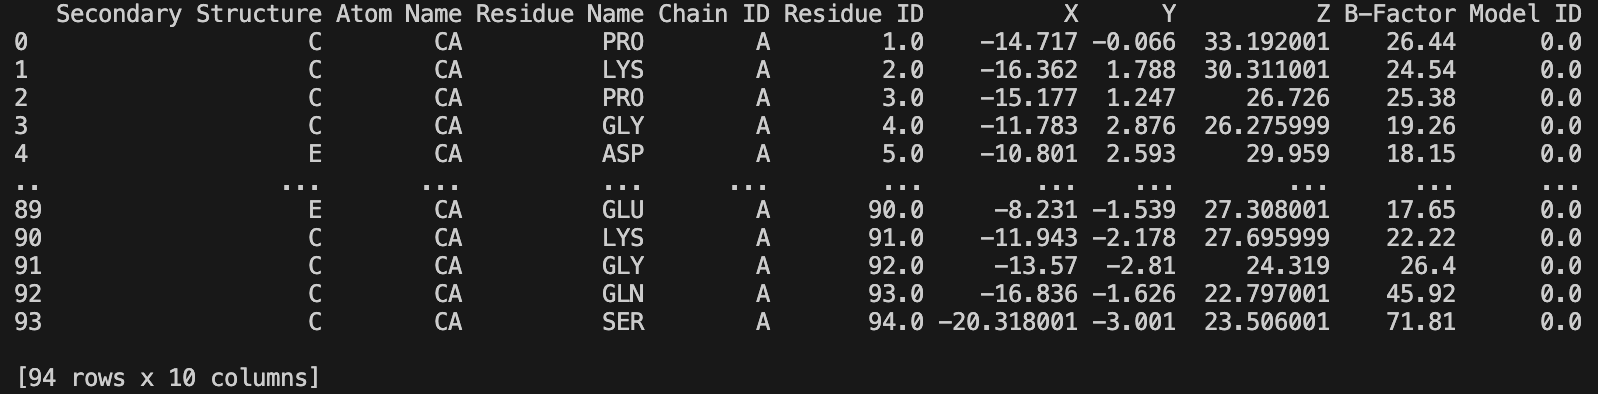
\includegraphics[width=0.8\textwidth]{/Users/enrico/PROTEINS/tesi/immagini_tesi_ingelse/Screenshot 2024-12-11 at 12.00.12.png
    }
    \caption{Dataset of 3LNX.}
\end{figure}
\begin{figure}[h!]
    \centering
    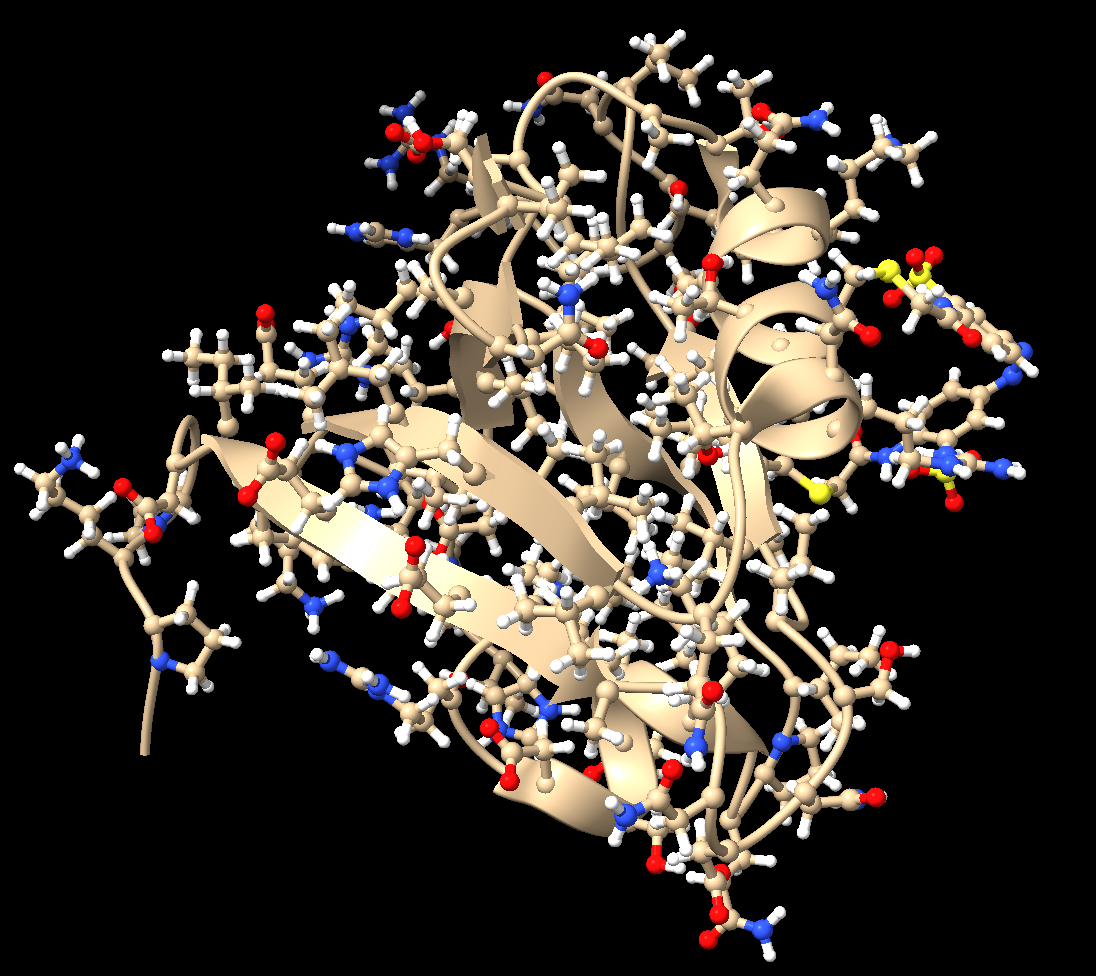
\includegraphics[width=0.8\textwidth]{/Users/enrico/PROTEINS/tesi/immagini_tesi_ingelse/Screenshot 2024-12-05 at 15.56.16.png}
    \caption{Representation of the 3LNX. Atoms are colored by element: O (red), N (blue), C (beige), and H (white). The yellow feature indicates the azobenzene moiety.}
\end{figure}

\noindent\textbf{Structural Highlights:}
\begin{itemize}
    \item \textbf{Overall Structure}: The PDZ domain of 3LNX contains multiple $\beta$-strands and $\alpha$-helices that create a canonical PDZ fold, complete with a characteristic ligand-binding groove.
    \item \textbf{Atomic Representation}: The azobenzene derivative is covalently attached, acting as a molecular photoswitch. Its isomerization influences the positioning of surrounding residues and the backbone conformation.
    \item \textbf{Functional Elements}: The ligand-binding groove is visible, providing insight into how photoswitching might modulate binding events by altering groove shape, depth, and accessibility.
\end{itemize}

\newpage
\section*{Connection Radius}

\noindent A critical aspect of analyzing 3LNX’s structural data is the choice of the connection radius when constructing the Kirchhoff matrix. 
This matrix forms the basis of GNM and is widely used to probe the collective motions within proteins.
By selecting an appropriate connection radius, one captures both local and long-range interactions between residues, ensuring that the resulting network accurately reflects the protein’s mechanical and dynamic properties.

\begin{figure}[h!]
    \centering
    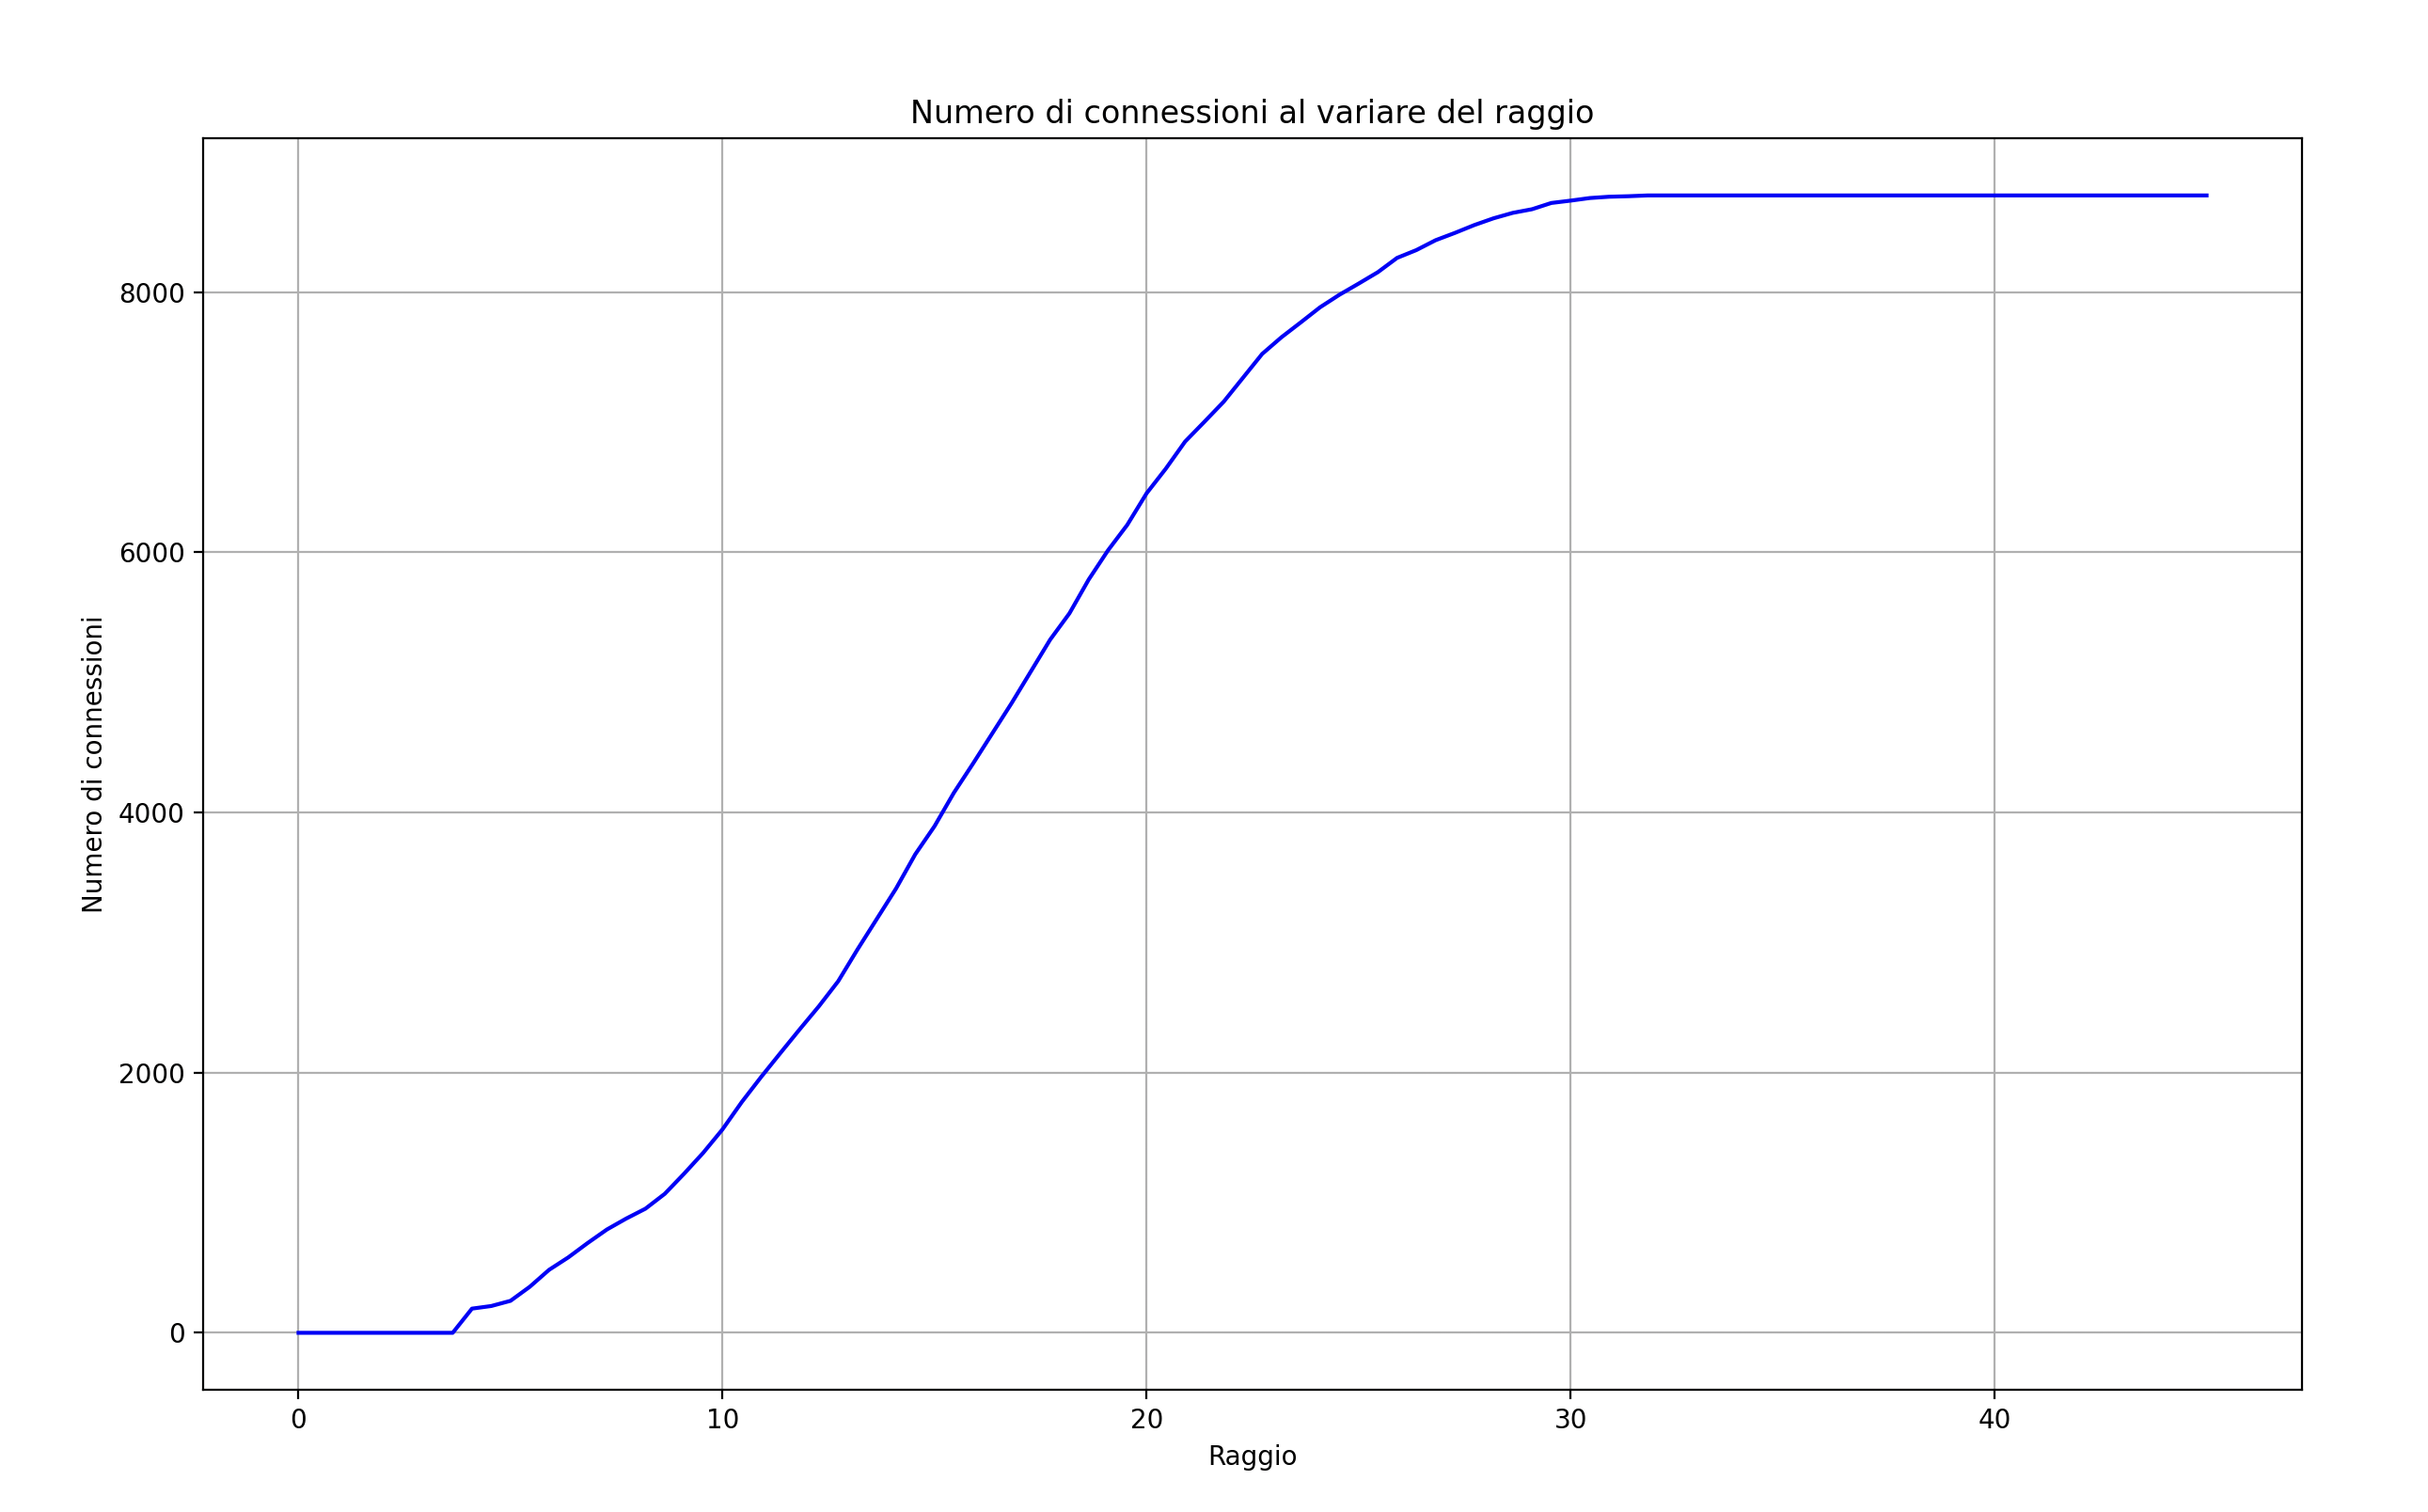
\includegraphics[width=0.8\textwidth]{/Users/enrico/PROTEINS/tesi/immagini_tesi_ingelse/Screenshot 2024-12-08 at 11.54.32.png}
    \caption{ Number of links in function of the connection radius.}
\end{figure}

It is common in litterature to take a value for the connection radius $\tilde{x} \approx \frac{1}{2} x^*, \text{ dove } x^* \text{ è tale che } f''(x) \big|_{x = x^*}$ = 0. In our case we took the value of 8.0 nm.\\
\begin{figure}[h!]
    \centering
    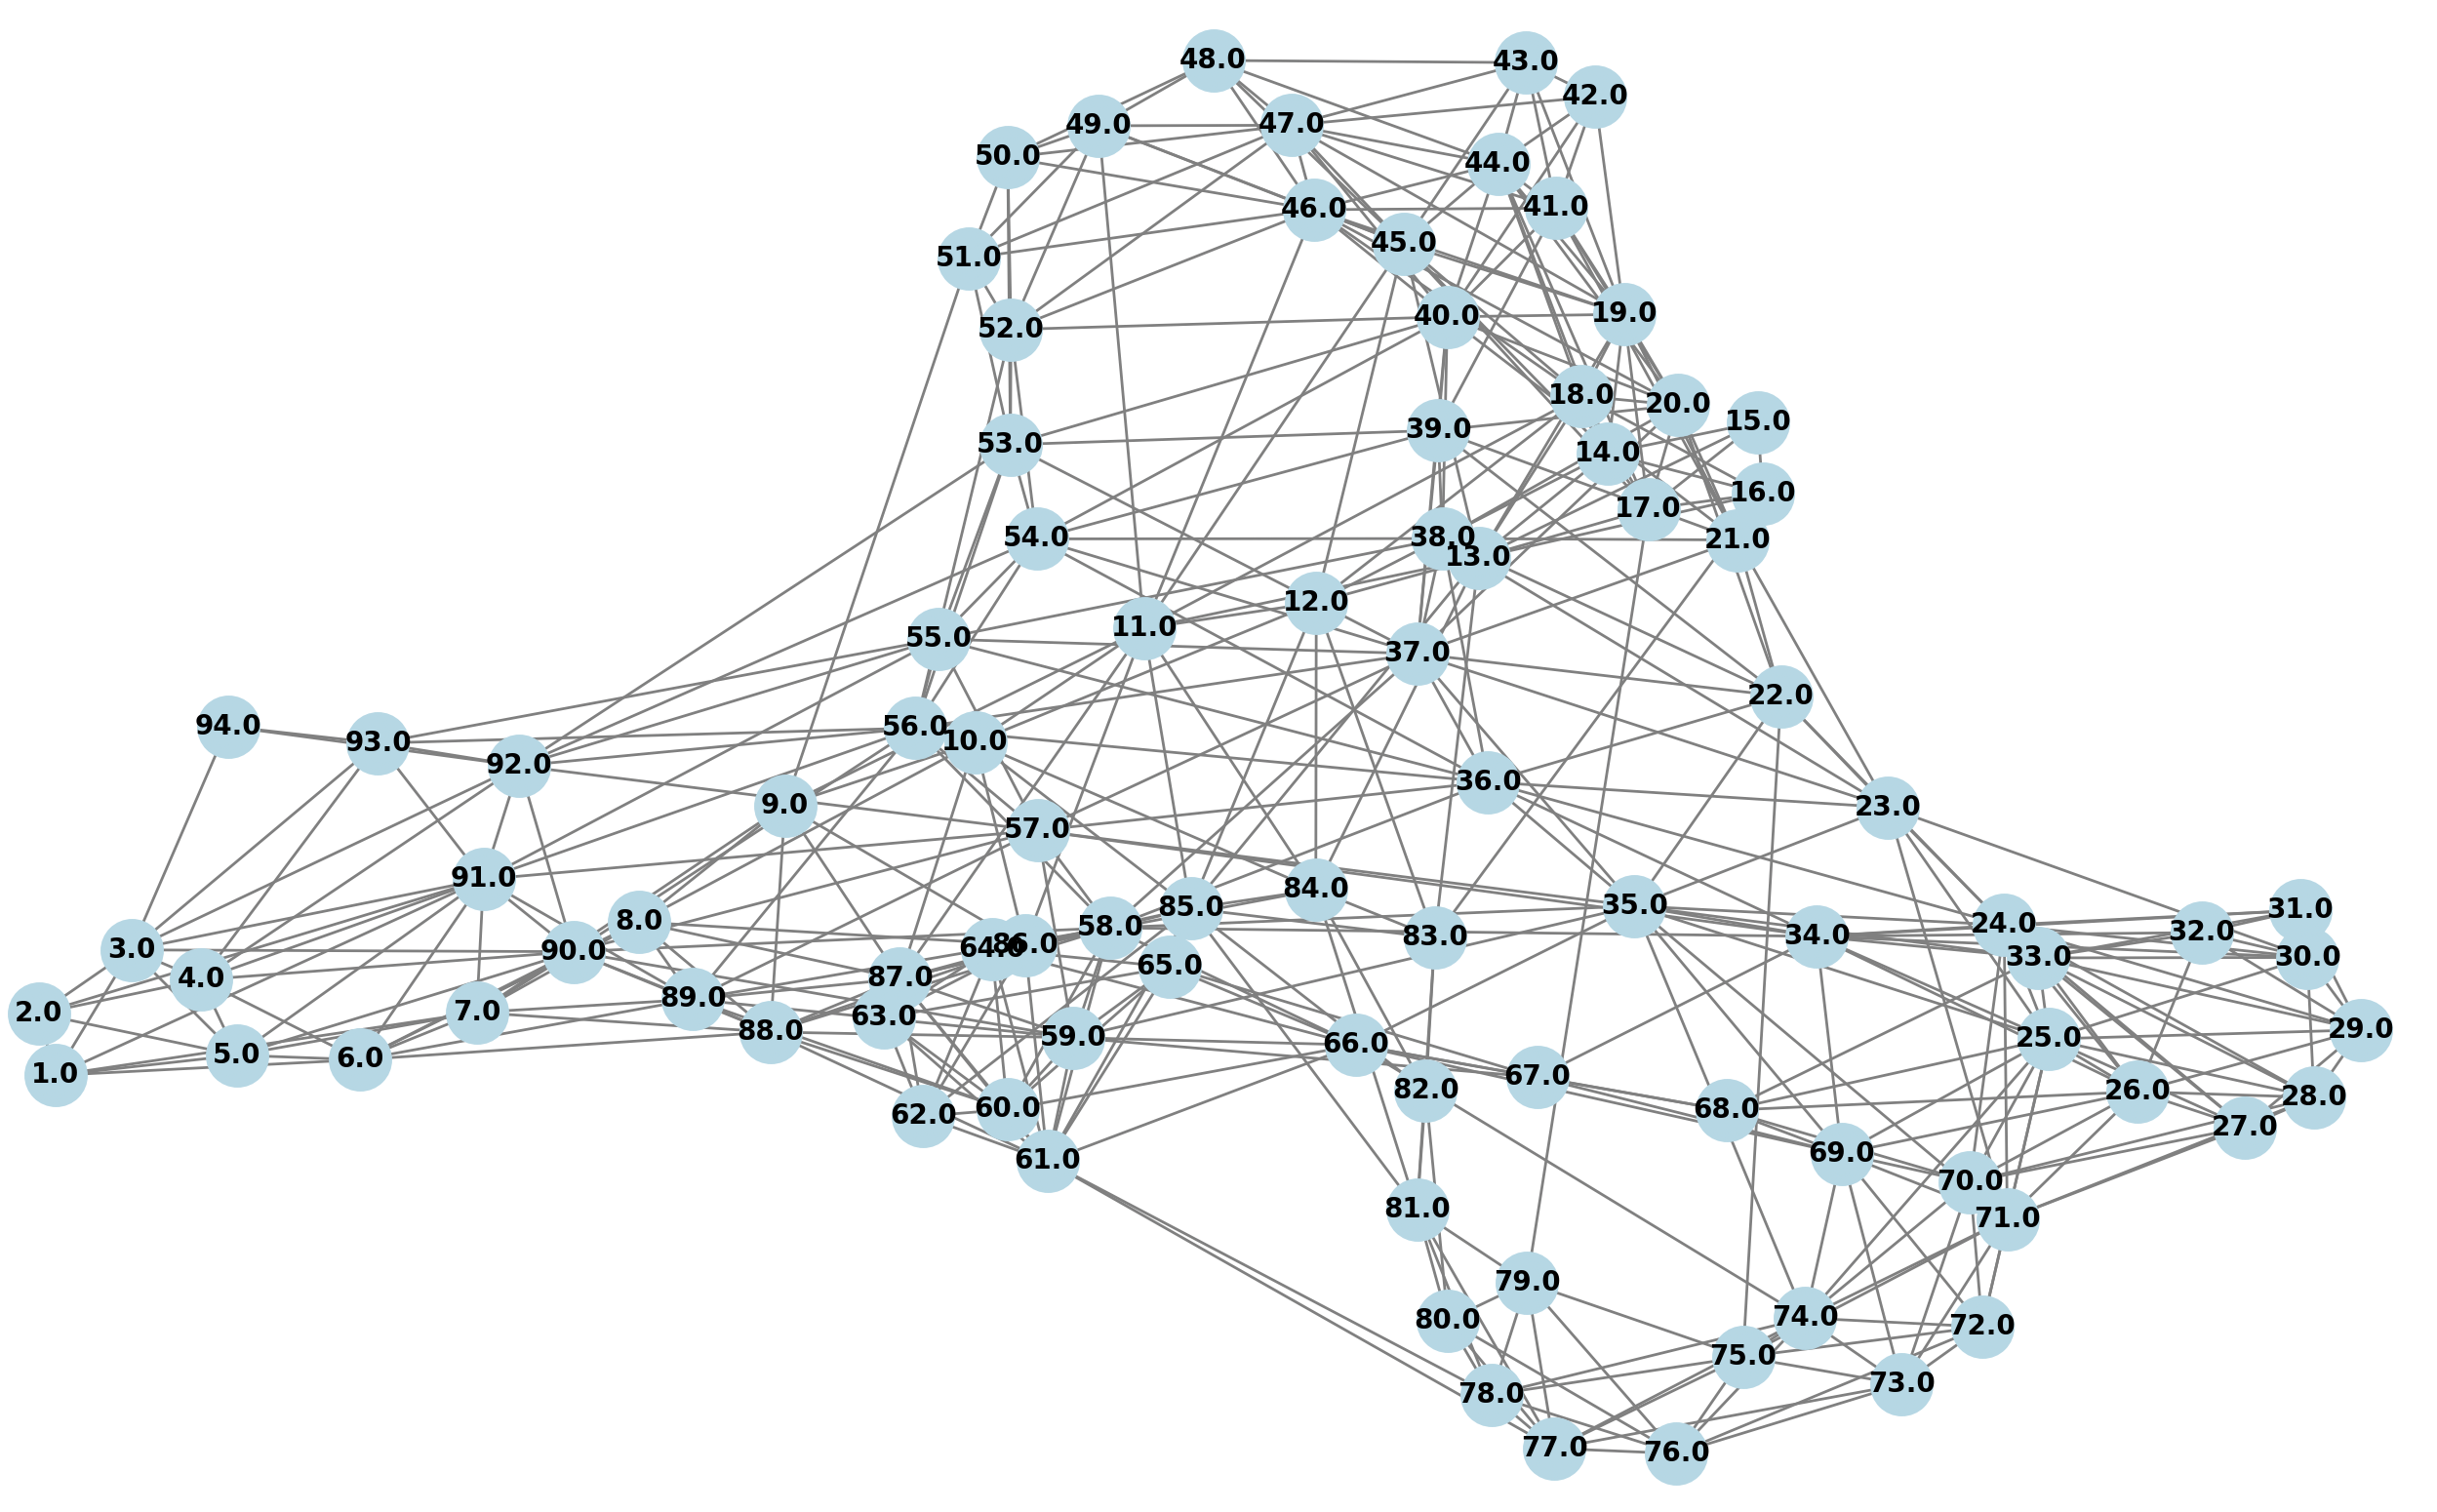
\includegraphics[width=0.8\textwidth]{/Users/enrico/PROTEINS/tesi/immagini_tesi_ingelse/Screenshot 2024-12-11 at 11.59.21.png}
    \caption{Bidirectional Graph obtained with radius of 8.0 .}
\end{figure}


\newpage
\section*{Kirchhoff Matrix}
\noindent Applying \eqref{Kirchhoff} to the protein structure, we obtain the Kirchhoff matrix \(\mathbf{K}\) for the system. This matrix captures the connectivity between residues and provides insights into the protein's structural dynamics. 
We choose to put the value of the link between two native pair (near neighbor), equal to 20, otherwise the link is equal to 1.
So:
Let \( G = (V, E) \) be a graph where \( V \) is the set of vertices and \( E \) is the set of edges. Define the weight of the link between two vertices \( i \) and \( j \) as \( w(i, j) \).

We assign weights as follows:
\[
w(i, j) =
\begin{cases}
20, & \text{if } i \text{ and } j \text{ are near neighbors}, \\
1, & \text{otherwise}.
\end{cases}
\]
The chosen weights are based on the relative importance of interactions in the context of protein stability and structural dynamics:
\paragraph{Near-neighbor interactions (native pairs):} \\
\textbf{Physical Basis:} Near neighbors are typically connected by strong covalent bonds or stabilized by dense non-covalent interactions (e.g., van der Waals forces, hydrogen bonds). These interactions dominate the local stability and rigidity of the protein structure.\\

\textbf{Quantitative Support:} The energy contributions from covalent bonds (300–400 kJ/mol) and closely packed van der Waals interactions are significantly higher than those from distant or weaker interactions.\\

\textbf{Weight Selection:} By assigning a weight of 20, we prioritize the influence of these dominant interactions in the Kirchhoff matrix. This ensures that the matrix reflects the critical role of local connectivity in determining the protein's overall structural stability.\\
\\
\paragraph{Distant interactions:}
\textbf{Physical Basis:} Residues that are not near neighbors may still interact through long-range forces (e.g., electrostatic or weak van der Waals forces). However, these interactions are generally less frequent and contribute less to the rigidity of the protein.

\textbf{Weight Selection:} Assigning a lower weight of 1 acknowledges the reduced importance of these interactions while still accounting for their presence in the protein network.
\begin{figure}[h!]
    \centering
    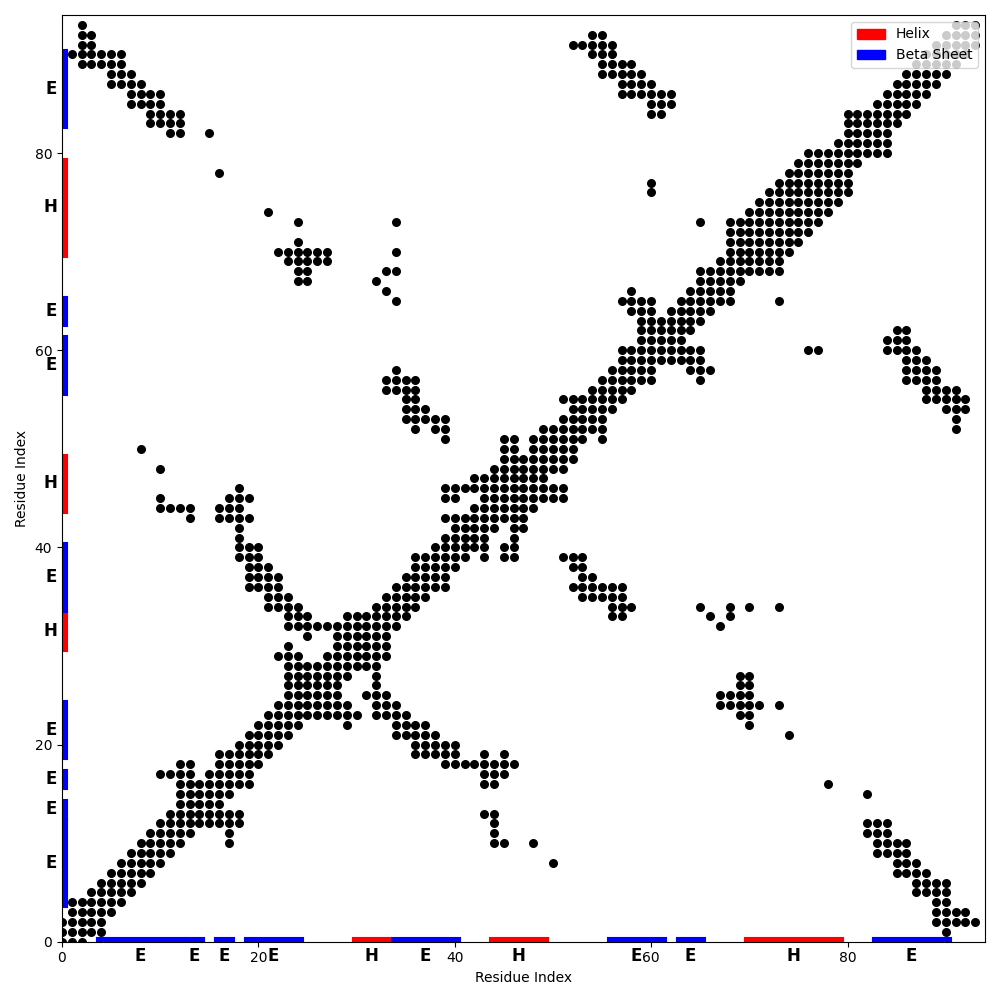
\includegraphics[width=0.8\textwidth]{/Users/enrico/PROTEINS/tesi/immagini_tesi_ingelse/Matrice di Kirchhoff della Proteina.png}
    \caption{Kirchoff Matrix.}
\end{figure}
\\\\\\\\\\\\\\

We notice first that as expected the Kirchhoff matrix is symmetric and that the diagonal elements are all negative. This is consistent with the physical interpretation of the matrix, where the diagonal elements represent the sum of the coupling strengths between a residue and all other residues in the protein. The negative sign indicates that the interactions are stabilizing, as expected in a protein structure. The off-diagonal elements represent the coupling between pairs of residues, reflecting the network of interactions that stabilize the protein's structure.
It is important to notice also that most of the links are between near residues, but we have also some cluster of links between distant residues. This is important because it means that the protein is not a simple chain of residues but it is a complex network of interactions.
\newpage



\section*{Correlation Matrix}
\noindent The two figures below illustrate the correlation matrices obtained from the protein structure. The elements of the matrix represent correlations between residues \(i\) and \(j\), derived from the dynamics and structure of the system. Overlaying the secondary structure (Helices: red; Beta Sheets: blue) helps to contextualize the correlations within structural motifs. The Kirchhoff matrix was used to compute these correlations.
\paragraph{Figure Analysis:}
\begin{itemize}
    \item \textbf{First Plot: Correlation Matrix (NaNs handled as False):}
    \begin{itemize}
        \item The red box highlights a region of strong local correlations, likely associated with tightly coupled residues within a helix or beta sheet structure.
        \item The light background suggests weak or negligible correlations outside the main diagonal and the highlighted regions, reflecting weaker interactions or dynamic decoupling.
        \item The diagonal dominance indicates strong correlations between residues within the same structural domain.
    \end{itemize}

    \item \textbf{Second Plot: Correlation Matrix (NaNs handled as True):}
    \begin{itemize}
        \item The overall structure appears more diffuse, with non-local correlations extending further from the diagonal.
        \item The red box again highlights a region of strong correlations, consistent with a structural motif (helix or beta sheet).
        \item The increased blue intensity in some regions may suggest the inclusion of weak, long-range interactions due to the handling of missing values (NaNs as True).
        \item Differences in the correlation intensity compared to the first plot reflect the impact of NaN handling on the computation of the correlation matrix.
    \end{itemize}
\end{itemize}

\paragraph{Relation to the Kirchhoff Matrix:}
The Kirchhoff matrix directly influences the correlation matrices by encoding the connectivity between residues. 
\begin{itemize}
    \item The strong correlations in the highlighted regions correspond to residues with high connectivity in the Kirchhoff matrix (near neighbors with weights of 20).
    \item Weaker correlations in the off-diagonal regions are consistent with weaker weights (1) assigned to distant interactions in the Kirchhoff matrix.
\end{itemize}

\begin{figure}[h!]
    \centering
    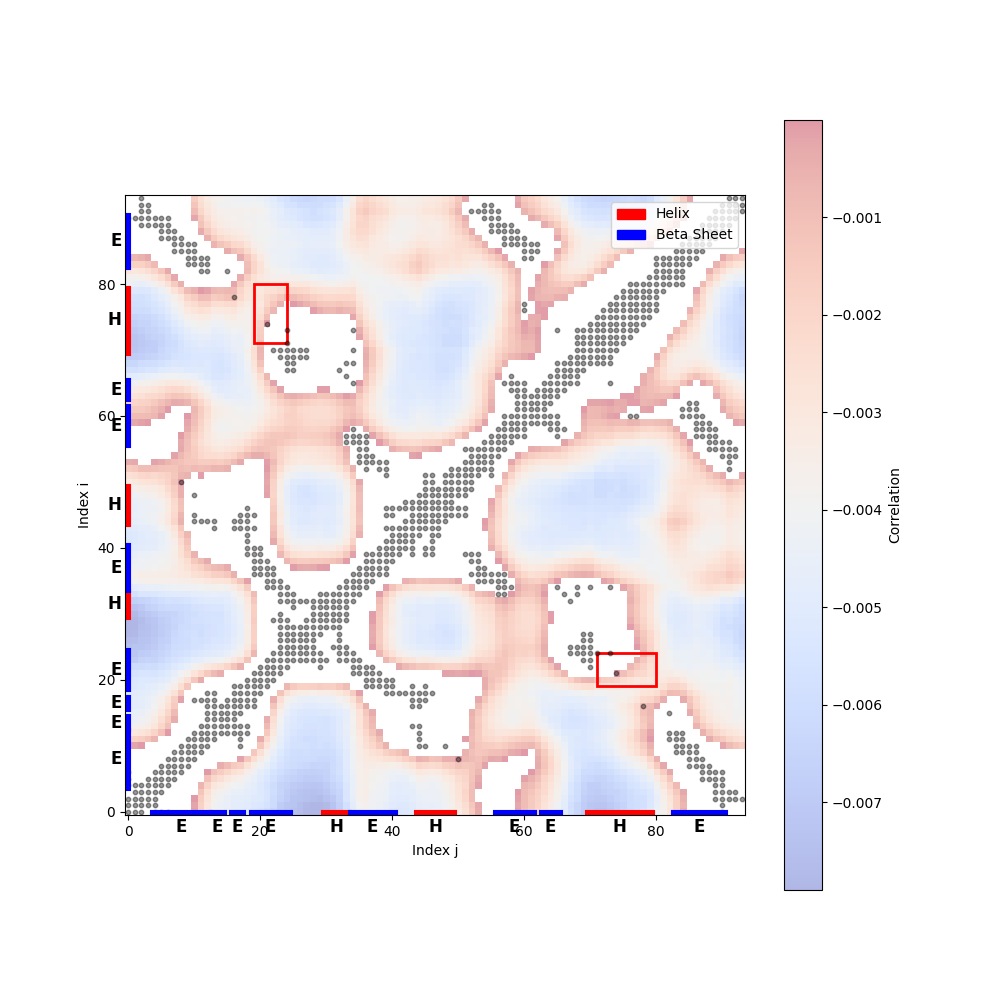
\includegraphics[width=0.8\textwidth]{/Users/enrico/PROTEINS/tesi/immagini_tesi_ingelse/Correlation_MatrixNan_False.png}
    \caption{Negative covariance between residues at time 0.}
\end{figure}
\begin{figure}[h!]
    \centering
    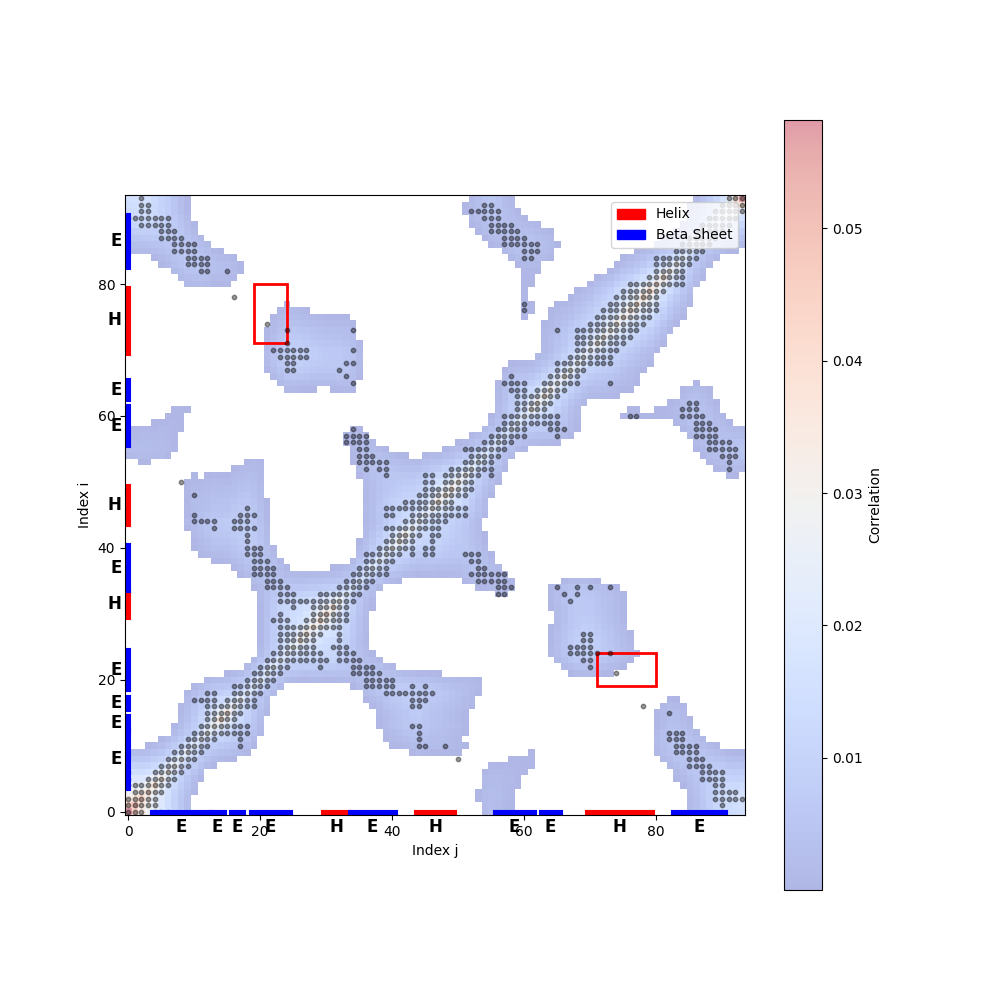
\includegraphics[width=0.8\textwidth]{/Users/enrico/PROTEINS/tesi/immagini_tesi_ingelse/Correlation_MatrixNan_True.png}
    \caption{Positive covariance between residues at time 0.}
\end{figure}

\newpage
\section*{Beta Factors}
\noindent The plot above compares the experimental \( B \)-factors (blue curve), as we said in \eqref{beta} $B_i = 8\pi^2 C_{ii}$, with the predicted \( B \)-factors (red curve) along the residue index. The \( B \)-factors, which represent the atomic displacement or flexibility, are a critical measure of the dynamic behavior of the protein structure.
\paragraph{Analysis:}
\begin{itemize}
    \item \textbf{Experimental \( B \)-factors (blue curve):}
    \begin{itemize}
        \item The blue curve shows regions of higher flexibility (peaks) and rigidity (troughs) as derived from experimental data.
        \item Peaks in the \( B \)-factors align with regions of loops or exposed residues, typically more flexible regions.
        \item Troughs align with structured regions such as helices or beta sheets, which are inherently more rigid.
    \end{itemize}

    \item \textbf{Predicted \( B \)-factors (red curve):}
    \begin{itemize}
        \item The predicted \( B \)-factors generally follow the experimental trend, demonstrating the effectiveness of the model in capturing the dynamics of the protein.
        \item Discrepancies between the predicted and experimental curves are visible in certain regions, particularly near residues with extreme flexibility or rigidity. These deviations may be due to limitations in the Kirchhoff matrix approximation or oversimplified assumptions in the modeling process.
    \end{itemize}
\end{itemize}
Using formula of section \ref{sec:Evaluation}, we can evaluate the model performance by calculating the Root Mean Squared Error (RMSE) and Mean Absolute Error (MAE) between the predicted and experimental \( B \)-factors. 
These metrics provide a quantitative assessment of the model's accuracy in capturing the protein's dynamic behavior.
\begin{table}[h!]
    \centering
    \begin{tabular}{|c|c|}
    \hline
    \textbf{Metric} & \textbf{Value} \\ \hline
    RMSE & 8.5200 \\ \hline
    MAE  & 6.4146 \\ \hline
    \end{tabular}
    \caption{Model Performance Metrics}
    \label{tab:model_metrics}
\end{table}




\paragraph{Secondary Structure Context:}
\begin{itemize}
    \item The background shading (red and blue bands) indicates secondary structure elements:
    \begin{itemize}
        \item \textbf{Red regions:} Helices, characterized by lower \( B \)-factors and greater rigidity.
        \item \textbf{Blue regions:} Beta sheets, which also exhibit lower \( B \)-factors compared to loops but slightly higher flexibility than helices.
    \end{itemize}
    \item The alignment of peaks and troughs in the \( B \)-factor curves with these shaded regions provides structural context to the observed dynamics.
\end{itemize}

\paragraph{Model Implications:}
\begin{itemize}
    \item The good agreement between experimental and predicted \( B \)-factors in structured regions (helices and beta sheets) supports the validity of the Kirchhoff matrix-based model.
    \item Discrepancies in loop regions suggest that additional factors, such as long-range interactions or local disorder, might need to be incorporated into the model for improved accuracy.
\end{itemize}

This analysis highlights the capability of the Kirchhoff matrix to predict protein flexibility while identifying areas for potential refinement.
\begin{figure}[h!]
    \centering
    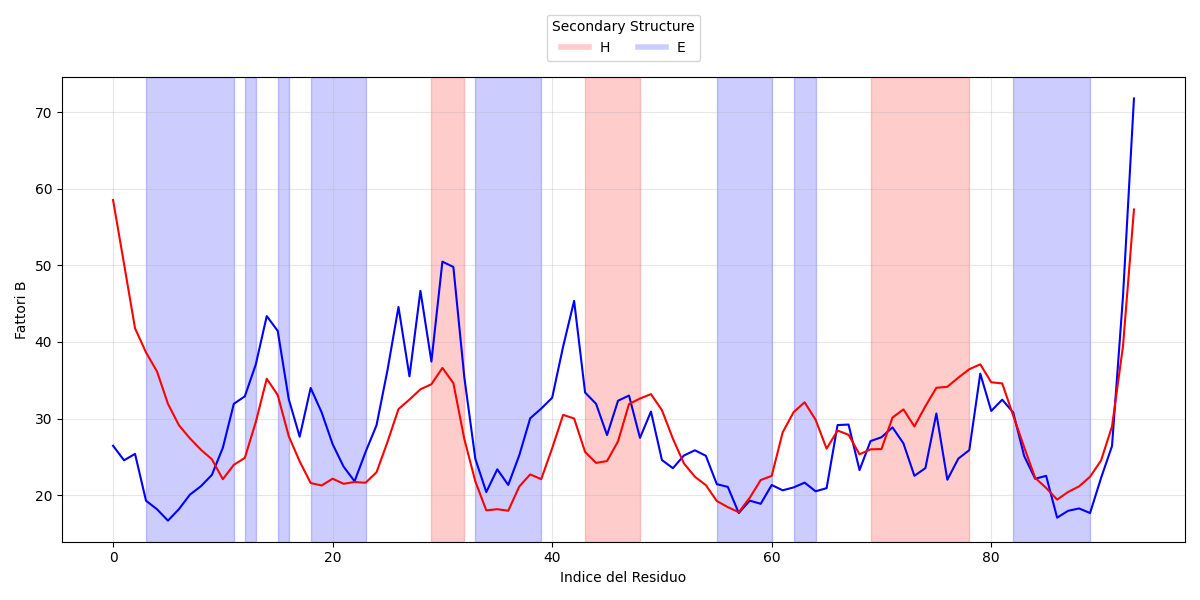
\includegraphics[width=0.8\textwidth]{/Users/enrico/PROTEINS/images/3LNX/beta_factors/Confronto_con_Struttura_Secondaria.png
    }
    \caption{Beta factors.}
\end{figure}



\newpage
\section*{Causal indicators in time}
\subsection*{Correlation in time}
\begin{figure}[h!]
    \centering
    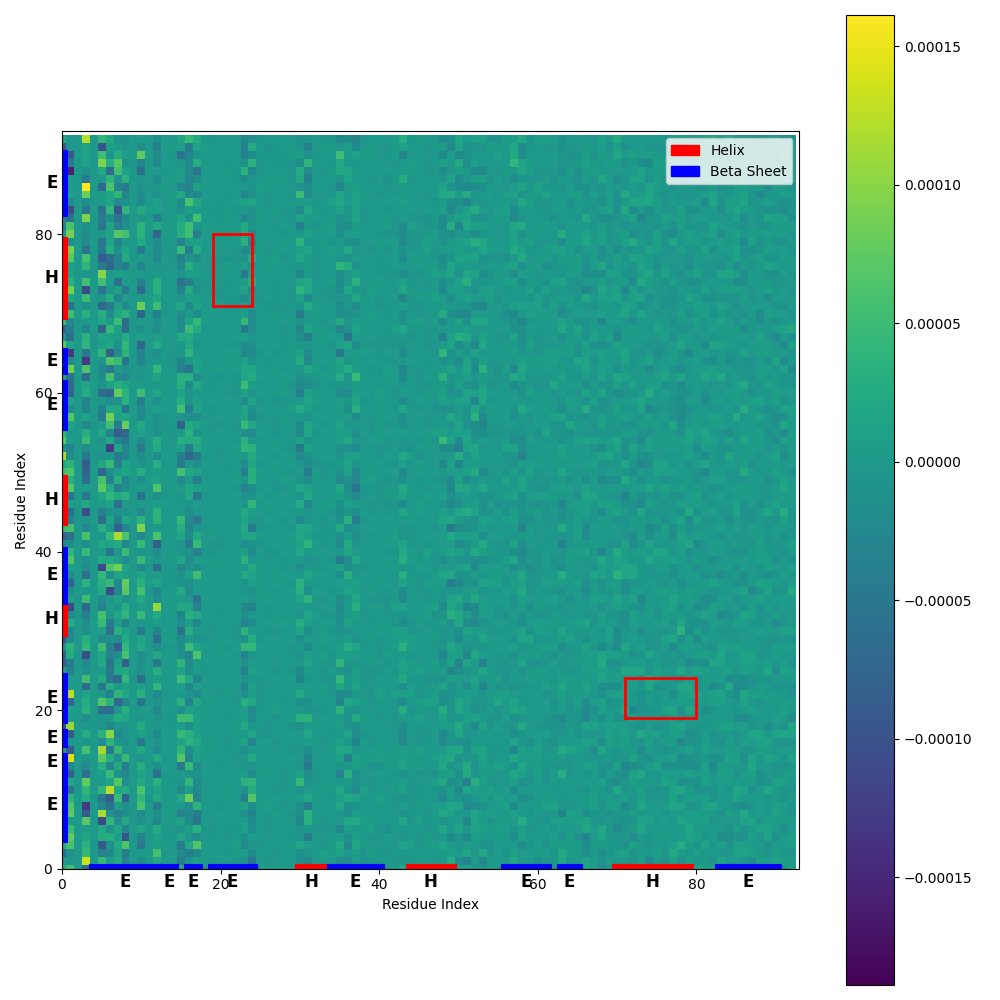
\includegraphics[width=0.8\textwidth]{/Users/enrico/PROTEINS/images/3LNX/Multiple_time_correlation/correlation.png}    
    \caption{Correlations in time.}
\end{figure}
\subsection*{Respones in time}
\begin{figure}[h!]
    \centering
    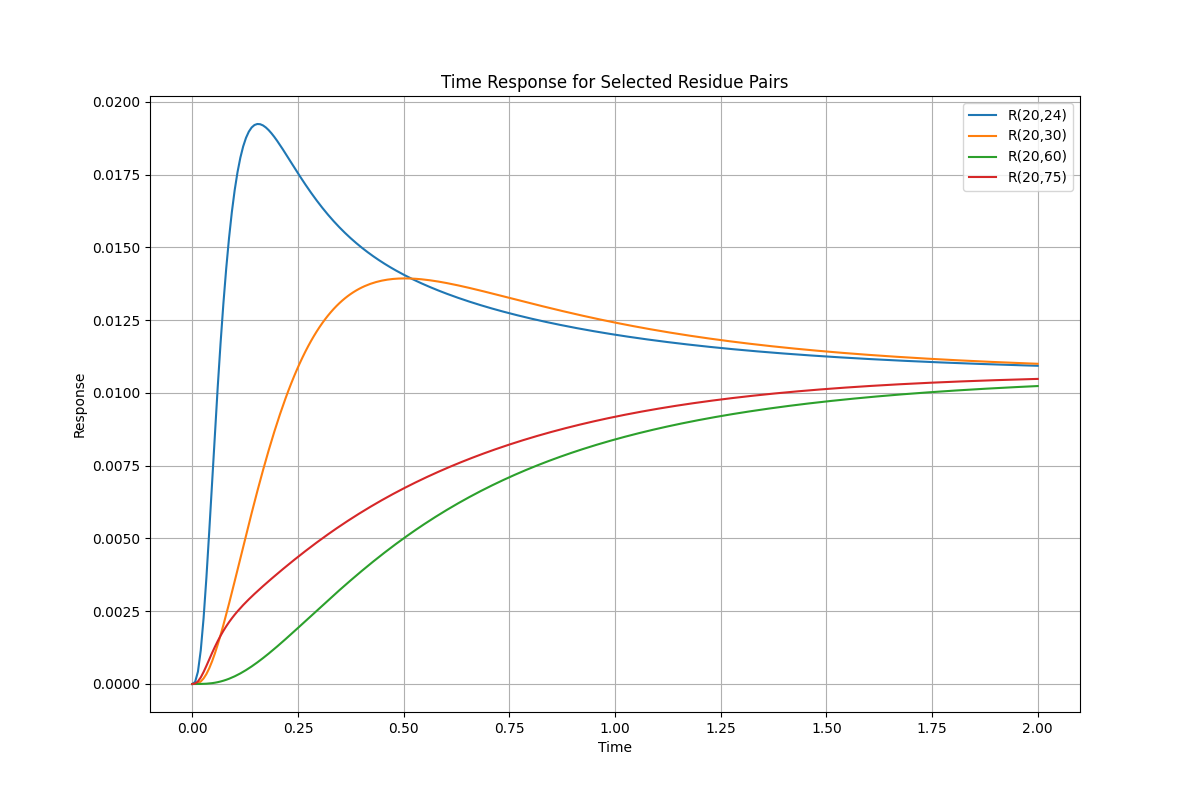
\includegraphics[width=0.8\textwidth]{/Users/enrico/PROTEINS/images/3LNX/Multiple_time_resposne/risposte.png}    
    \caption{Responses in time.}
\end{figure}
\subsection*{Transfer entropy in time}
\begin{figure}[h!]
    \centering
    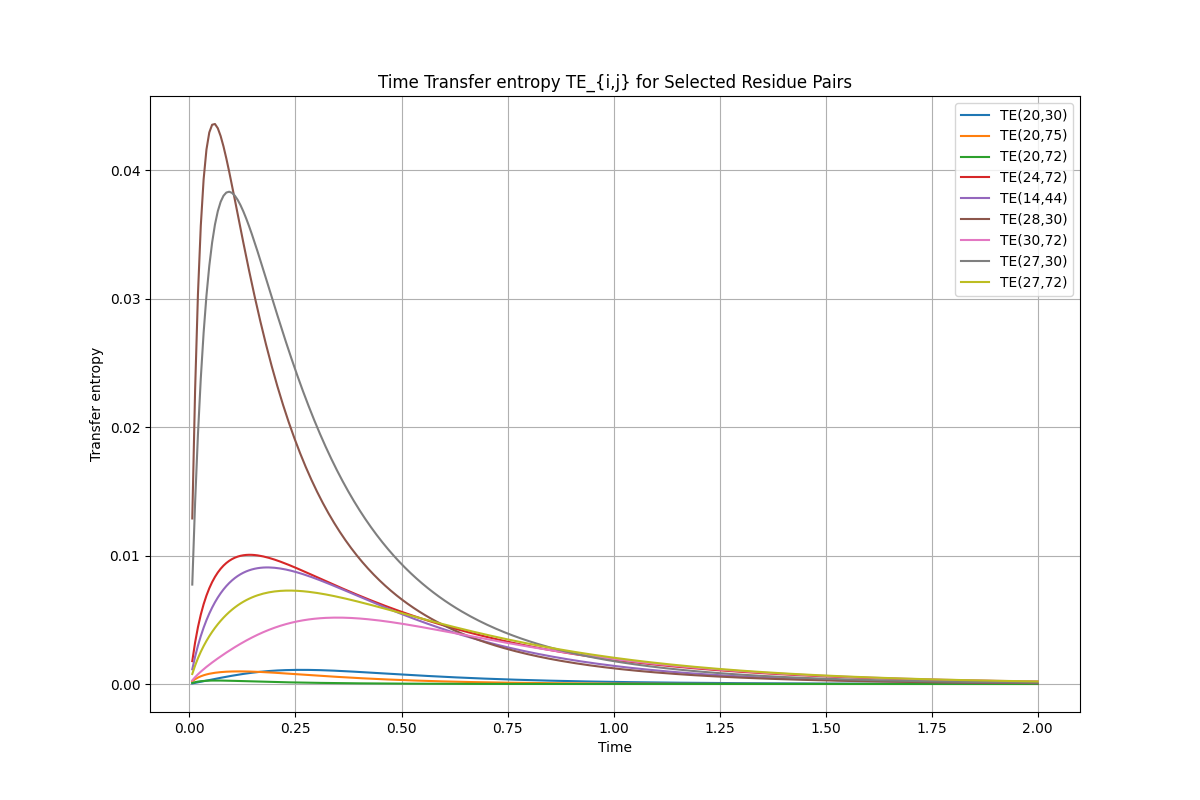
\includegraphics[width=0.8\textwidth]{/Users/enrico/PROTEINS/images/3LNX/Multiple_time_correlation/entropy.png}    
    \caption{Transfer entropy  in time.}
\end{figure}



\newpage
\section*{Causal indicators between residues}
\subsection*{characteristic time determination}
To analyze our system, it is essential to focus on timescales around the \textit{characteristic time} \(\tau\). 
If the time \(t\) is too small, the dynamics of the system cannot be observed effectively. Conversely, if \(t\) is too large, the relaxation behavior of the system becomes indistinguishable.

We can determine the characteristic time \(\tau\) of the system using the following algorithm:
\begin{enumerate}
    \item Compute the autocorrelation function \(C_{i,i}(t)\) for all available times \(t\).
    \item Identify, for each \(i\), the time \(t_i\) such that 
    \[
    C_{i,i}(t_i) = e^{-1} C_{i,i}(0),
    \]
    where \(C_{i,i}(0)\) represents the initial autocorrelation value.
    \item Calculate the mean of all \(t_i\). This mean value represents the characteristic time \(\tau\) of the system:
    \[
    \tau = \frac{1}{N} \sum_{i=1}^{N} t_i.
    \]
\end{enumerate}

\begin{figure}[h!]
    \centering
    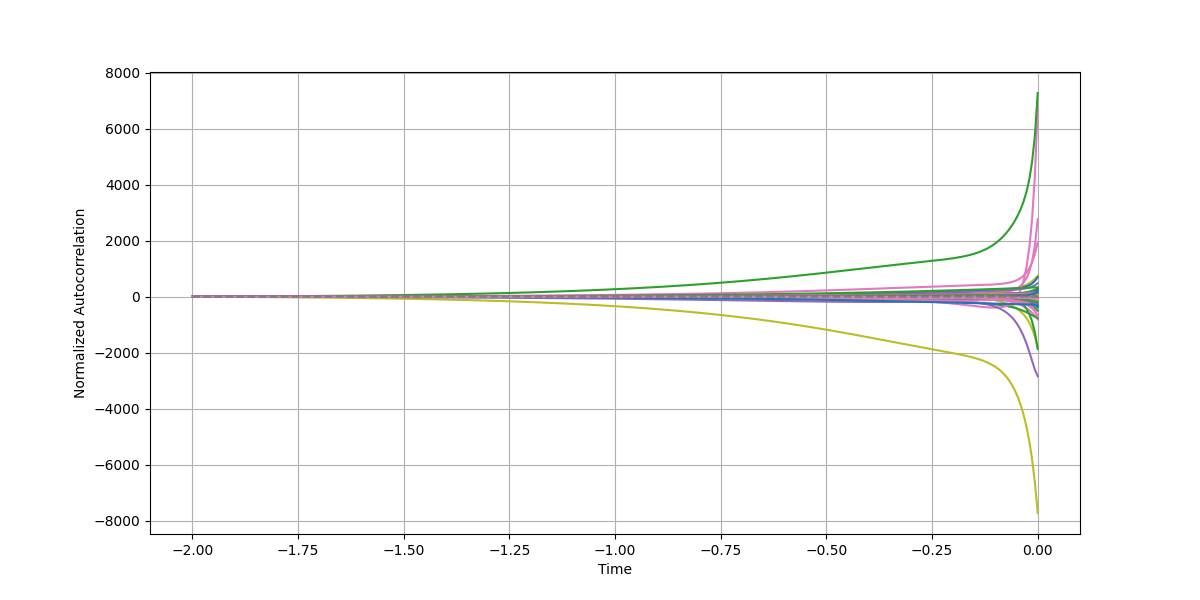
\includegraphics[width=0.8\textwidth]{/Users/enrico/PROTEINS/images/3LNX/Stima_tau/autocorrelation_fits.png}
    \caption{Fit of tau.}
\end{figure}
All the following analysis will be done around the characteristic time \(\tau\), specifically at [\(\tau\)-0.5*\(\tau\),\(\tau\),\(\tau\)+0.5*\(\tau\)].

\newpage



\subsection*{Correlation between residues}
\noindent The dynamic interplay between the beta sheet and the helix is quantitatively evident across all figures. The beta sheet stabilizes the protein through localized rigidity and strong intra-regional dynamics, while the helix introduces flexibility and facilitates long-range communication. These complementary roles are essential for balancing the stability and functional adaptability of the protein structure.

\begin{figure}[h!]
    \centering
    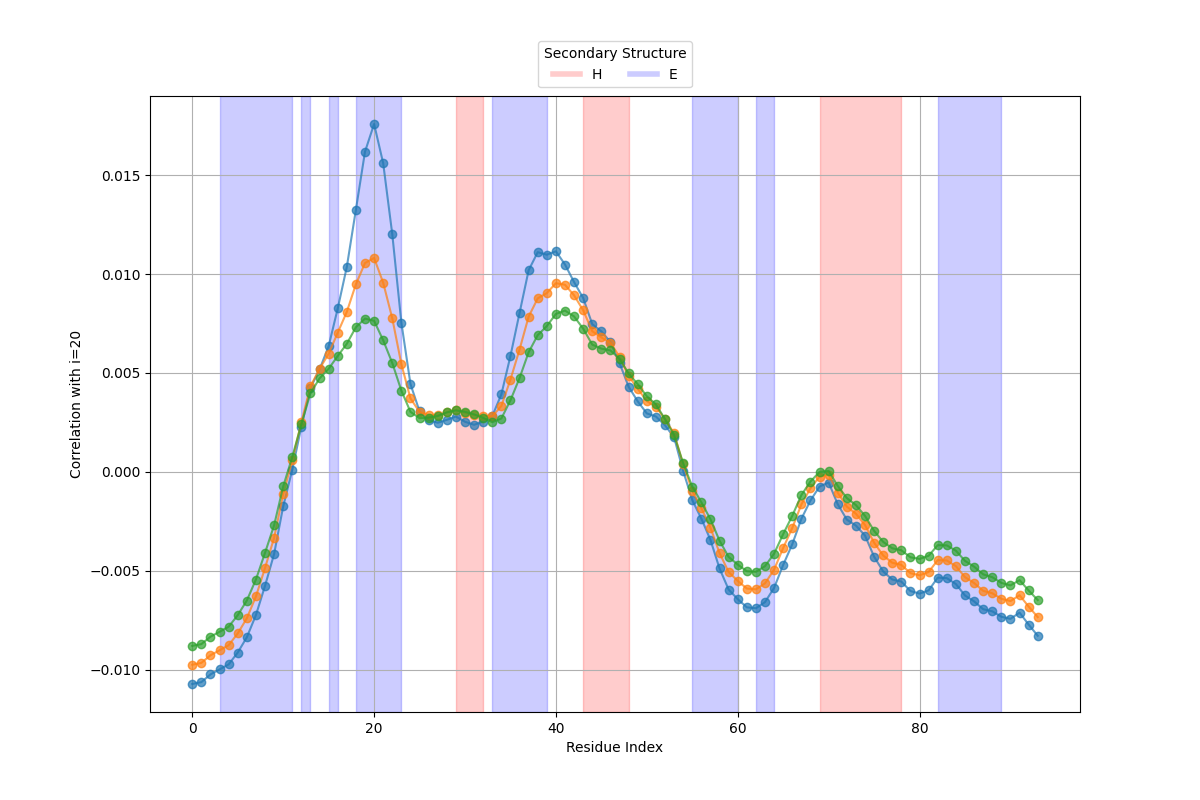
\includegraphics[width=0.8\textwidth]{/Users/enrico/PROTEINS/images/3LNX/Time_indicators/Residual Correlation C_ij for i=20 as a function of j at time index 0.png}
    \caption{Correlation perturbating 21-th residue.}
    \label{fig:corr21}
\end{figure}

\begin{figure}[h!]
    \centering
    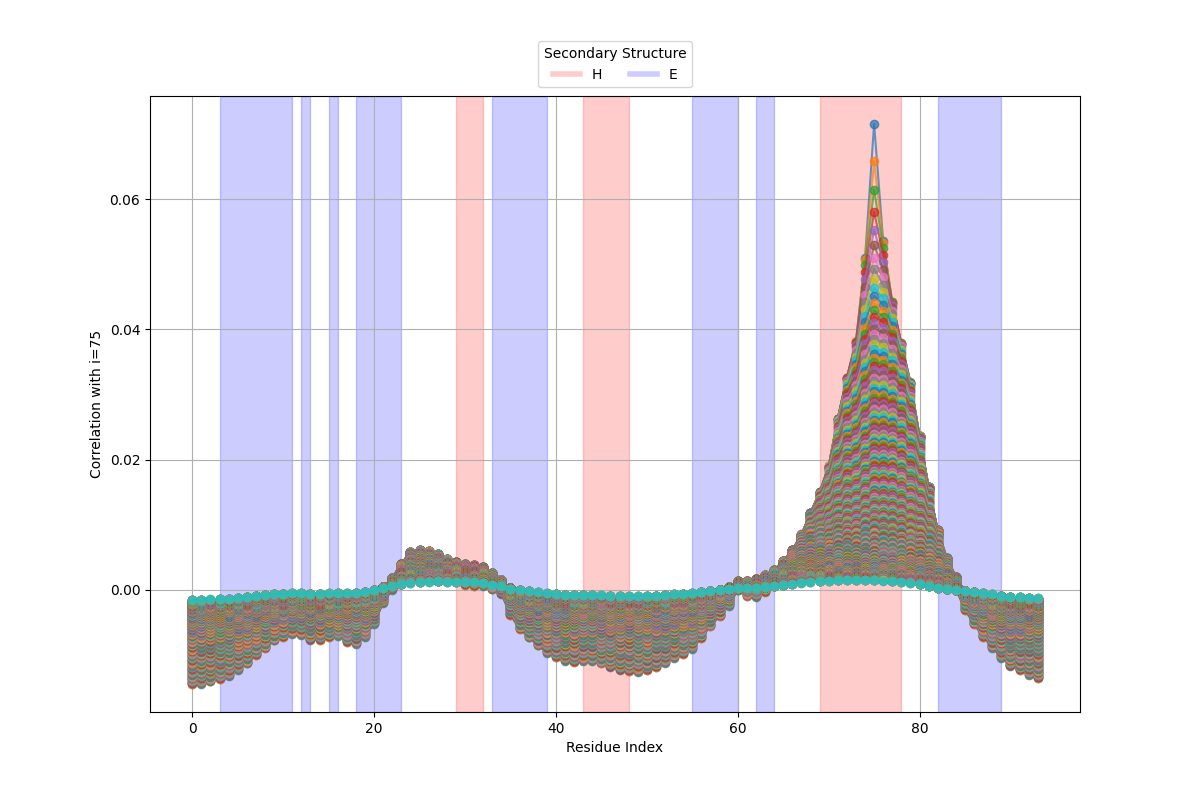
\includegraphics[width=0.8\textwidth]{/Users/enrico/PROTEINS/images/3LNX/Time_indicators/Residual Correlation C_ij for i=75 as a function of j at time index 0.png}
    \caption{Correlation perturbating 76-th residue.}
    \label{fig:corr76}
\end{figure}
\subsubsection*{Graphic analysis of correlation}
The figures provide a detailed view of the dynamic properties of the protein structure, focusing on the beta sheet around residue ~20 and the alpha helix near residue ~75. These secondary structures exhibit distinct dynamical behaviors, which are quantified using metrics such as inverse first mean time, correlation, response, and transfer entropy.
\paragraph{Figure \ref{fig:corr21}: Correlation with Residue ~20}

\begin{itemize}
    \item \textbf{Beta Sheet Region (Residue ~20):} Strong correlation values are observed in this region, reflecting the tightly coupled dynamics among the residues in the beta sheet. These high correlations are a direct consequence of the stabilizing hydrogen bonds that link the beta strands, enforcing collective motion within this region.
    \item \textbf{Alpha Helix Region (Residue ~75):} Moderate correlation values in the helix region suggest that residues near residue 75 are influenced by, but less directly connected to, the beta sheet. The helix's intrinsic flexibility reduces the strength of its correlation with the beta sheet residues.
    \item \textbf{Interpretation:} This figure emphasizes the beta sheet's role as a hub of strong dynamic interactions, anchoring the protein’s motion. The helix, while dynamically active, plays a more peripheral role in interacting with the beta sheet.
\end{itemize}

\paragraph{Figure \ref{fig:corr76}: Correlation with Residue ~75}
\begin{itemize}
    \item \textbf{Beta Sheet Region (Residue ~20):} Lower correlation values between the beta sheet and residue 75 indicate that the beta sheet's rigidity limits its dynamic communication with the helix. This suggests that the beta sheet’s motion is more self-contained, reducing its coupling to distant regions like the helix.
    \item \textbf{Alpha Helix Region (Residue ~75):} High correlation values around residue 75 highlight the helix's central role in propagating dynamic signals within the protein. These correlations reflect the helix’s ability to communicate dynamically with both nearby residues and more distant regions.
    \item \textbf{Interpretation:} The helix serves as a dynamic mediator, interacting more strongly with distant residues compared to the beta sheet. This figure underscores the helix’s flexibility and its role in bridging different structural regions of the protein.
\end{itemize}

\newpage
\newpage









\subsection*{Response between residues}
\begin{figure}[h!]
    \centering
    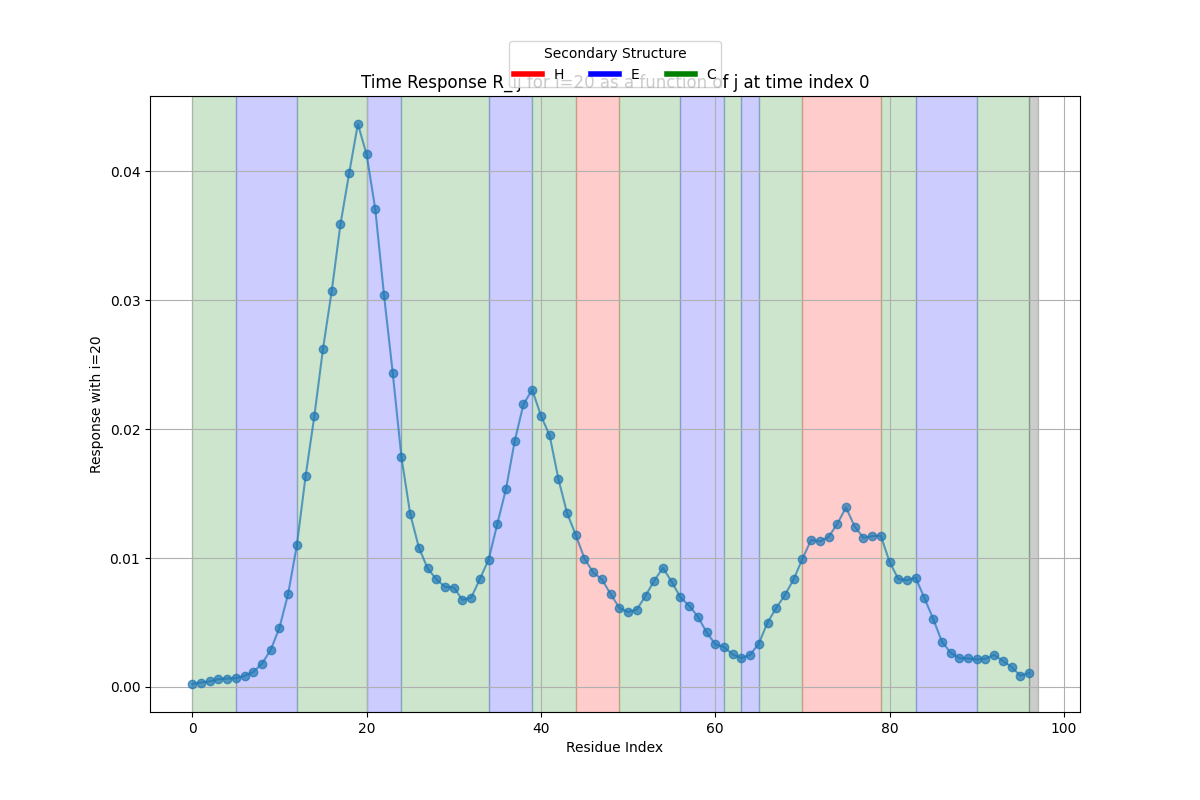
\includegraphics[width=0.8\textwidth]{/Users/enrico/PROTEINS/images/3LNX/Time_indicators/Time Response R_ij for i=20 as a function of j at time index 0.png}
    \caption{Response perturbating 21-th residue.}
    \label{fig:resp21}
\end{figure}


\begin{figure}[h!]
    \centering
    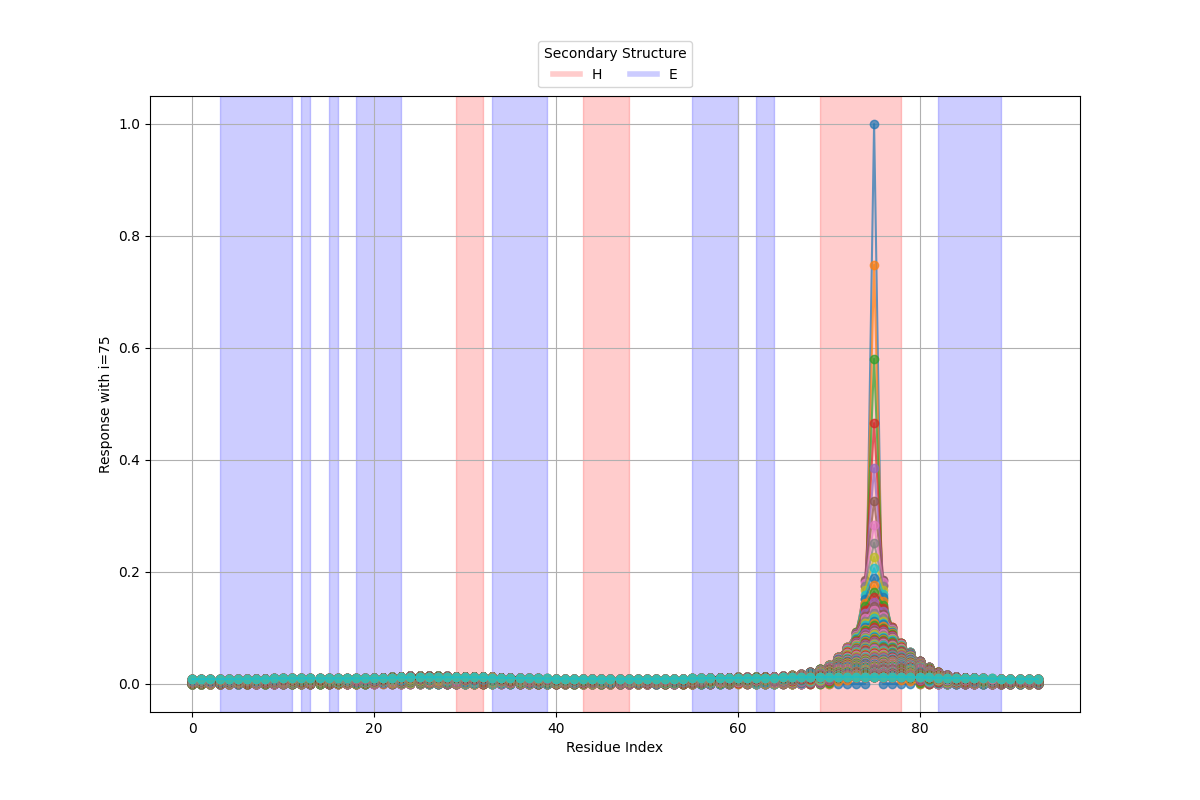
\includegraphics[width=0.8\textwidth]{/Users/enrico/PROTEINS/images/3LNX/Time_indicators/Time Response R_ij for i=75 as a function of j at time index 0.png}
    \caption{Response perturbating 76-th residue.}
    \label{fig:resp76}
\end{figure}
\subsubsection*{Graphic analysis of response}
\paragraph{Figure \ref{fig:resp21} : Response with Residue ~20}
\begin{itemize}
    \item \textbf{Beta Sheet Region (Residue ~20):} The response values around residue 20 show a sharp peak, consistent with the beta sheet's stabilizing influence on the protein's dynamics. The high response values highlight the beta sheet’s role in shaping the local dynamic environment.
    \item \textbf{Alpha Helix Region (Residue ~75):} In the helix region, the response to residue 20 is weaker, indicating that the helix dynamics are less directly influenced by the beta sheet. The helix's intrinsic flexibility decouples it from the rigid motions of the beta sheet.
    \item \textbf{Interpretation:} The beta sheet acts as a localized stabilizing force, with its influence tapering off in regions like the helix. This behavior supports the protein's need for both localized rigidity and broader adaptability.
\end{itemize}

\paragraph{Figure \ref{fig:resp76}: Response with Residue ~75}
\begin{itemize}
    \item \textbf{Beta Sheet Region (Residue ~20):} A weak response is observed in the beta sheet, consistent with its rigidity and lower susceptibility to dynamic signals originating from the helix.
    \item \textbf{Alpha Helix Region (Residue ~75):} A strong response peak near residue 75 reflects the helix's active role in facilitating dynamic transitions and responding to perturbations.
    \item \textbf{Interpretation:} The helix is a key dynamic element, complementing the beta sheet's rigidity by enabling dynamic adaptability and communication across the protein.
\end{itemize}



\newpage
\newpage









\subsection*{Transfer entropy between residues}
\begin{figure}[h!]
    \centering
    % Prima sottografia
    \begin{subfigure}[t]{0.48\textwidth}
        \centering
        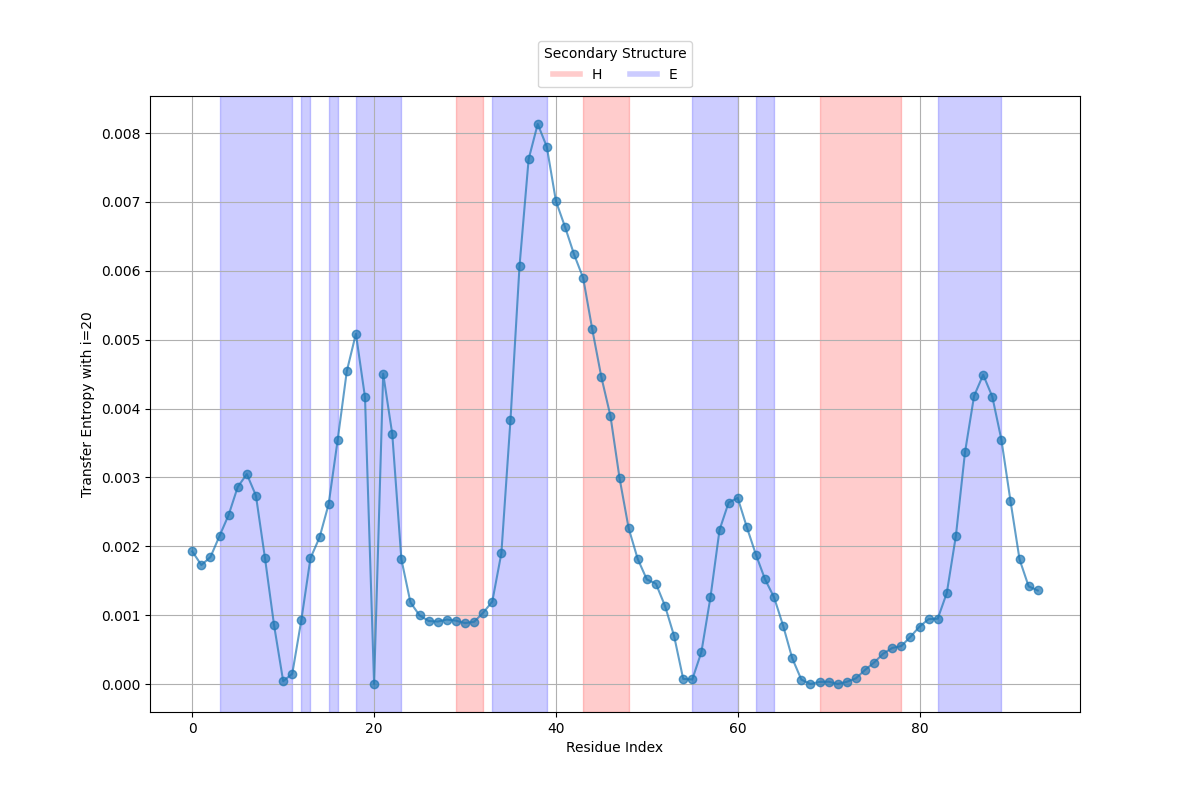
\includegraphics[width=\textwidth]{/Users/enrico/PROTEINS/images/3LNX/Time_indicators/Transfer Entropy TE_ij for i=20 as a function of j at time index 0.png}
        \caption{Transfer Entropy (j->21) ($TE_{21,j}$) perturbating 21-th residue.}
        \label{fig:TE21_i_j}
    \end{subfigure}
    \hfill
    % Seconda sottografia
    \begin{subfigure}[t]{0.48\textwidth}
        \centering
        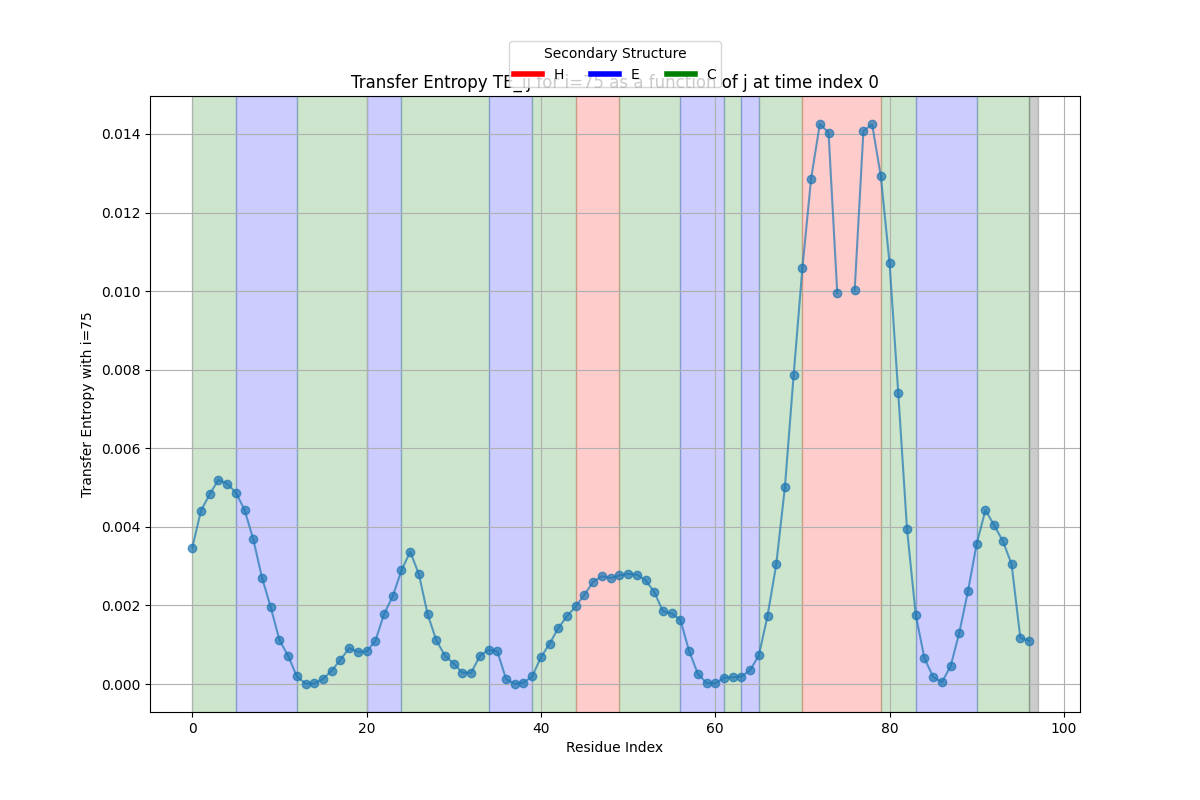
\includegraphics[width=\textwidth]{/Users/enrico/PROTEINS/images/3LNX/Time_indicators/Transfer Entropy TE_ij for i=75 as a function of j at time index 0.png}
        \caption{Transfer Entropy (j->76) ($TE_{76,j}$) perturbating 76-th residue.}
        \label{fig:TE76_i_j}
    \end{subfigure}
    \caption{Comparison of Transfer Entropy for different perturbated residues.}
    \label{fig:TE_comparison_i_j}
\end{figure}

\begin{figure}[h!]
    \centering
    % Prima sottografia
    \begin{subfigure}[t]{0.48\textwidth}
        \centering
        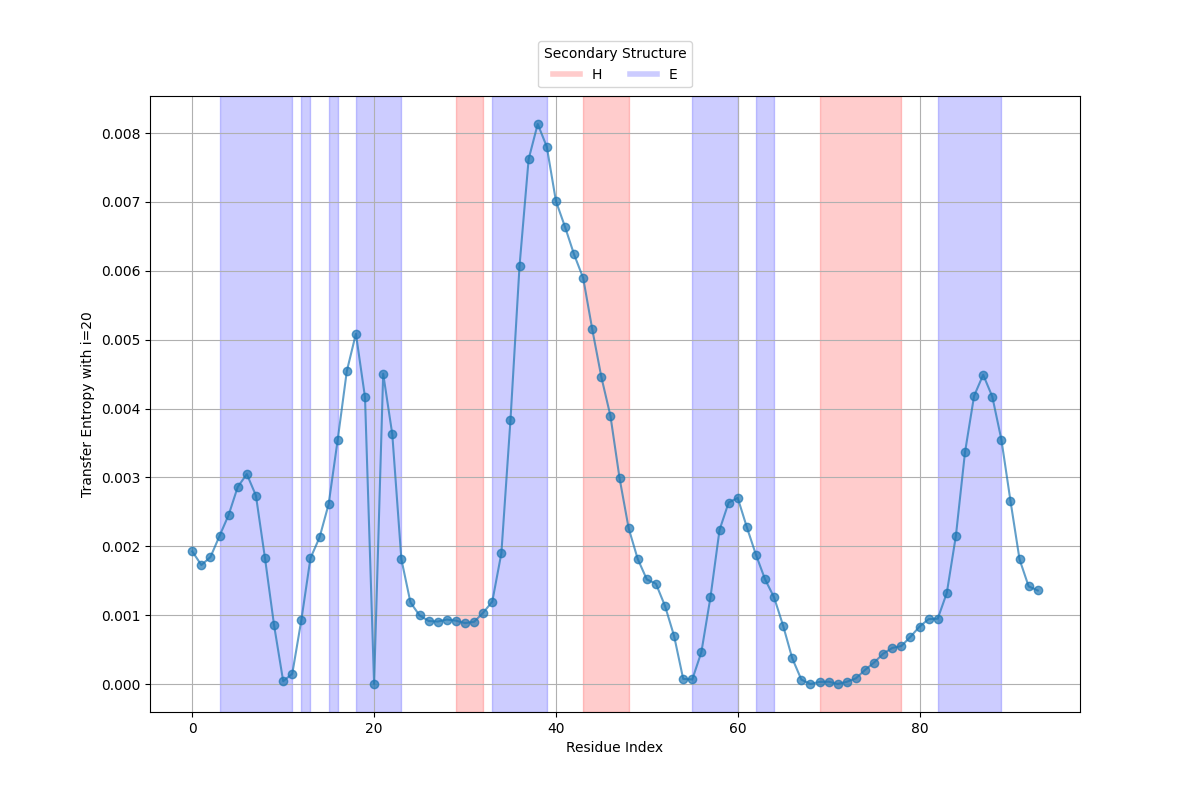
\includegraphics[width=\textwidth]{/Users/enrico/PROTEINS/images/3LNX/Time_indicators/Transfer Entropy TE_ji for i=20 as a function of j at time index 0.png}
        \caption{Transfer Entropy (21->j) ($TE_{j,21}$) perturbating 21-th residue.}
        \label{fig:TE21_j_i}
    \end{subfigure}
    \hfill
    % Seconda sottografia
    \begin{subfigure}[t]{0.48\textwidth}
        \centering
        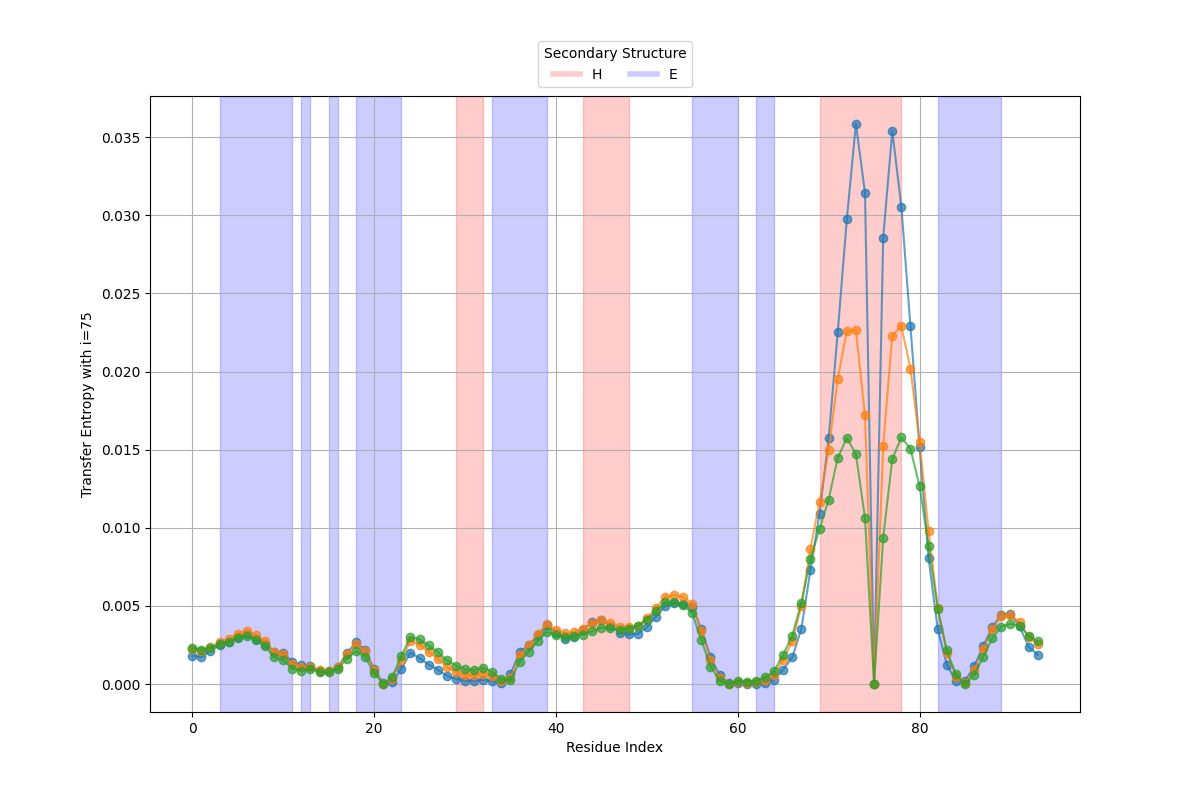
\includegraphics[width=\textwidth]{/Users/enrico/PROTEINS/images/3LNX/Time_indicators/Transfer Entropy TE_ji for i=75 as a function of j at time index 0.png}
        \caption{Transfer Entropy (76->j) ($TE_{j,76}$) perturbating 76-th residue.}
        \label{fig:TE76_j_i}
    \end{subfigure}
    \caption{Comparison of Transfer Entropy for perturbations affecting different residues (j<-i).}
    \label{fig:TE_comparison_j_i}
\end{figure}


\subsubsection*{Graphic analysis of transfer entropy}
\paragraph{Figure \ref{fig:TE_comparison_i_j}: Transfer Entropy with Residue ~20}
\begin{itemize}
    \item \textbf{Beta Sheet Region (Residue ~20):} High transfer entropy values in the beta sheet reflect strong localized information flow, emphasizing the beta sheet's role in stabilizing and coordinating motions within its region.
    \item \textbf{Alpha Helix Region (Residue ~75):} The helix shows lower transfer entropy values, indicating that it is less dynamically influenced by residue 20. This highlights the beta sheet's role as a local stabilizer rather than a global signal mediator.
    \item \textbf{Interpretation:} The beta sheet governs local dynamics through strong information flow, while the helix remains relatively decoupled in terms of direct influence.
\end{itemize}

\paragraph{Figure \ref{fig:TE_comparison_j_i}: Transfer Entropy with Residue ~75}
\begin{itemize}
    \item \textbf{Beta Sheet Region (Residue ~20):} Transfer entropy values indicate weak information flow from the helix to the beta sheet, consistent with the beta sheet's structural rigidity and localized dynamics.
    \item \textbf{Alpha Helix Region (Residue ~75):} Strong peaks in transfer entropy around residue 75 highlight its role in propagating dynamic information across the protein, making it a key mediator of long-range communication.
    \item \textbf{Interpretation:} The helix complements the beta sheet by actively facilitating dynamic interactions and communication throughout the protein.
\end{itemize}



\newpage
\newpage
\chapter{Conclusions Statical aprt}


\chapter{Conclusions}



\subsection*{NON METTEERLO Mean First time passage}
\begin{figure}[h!]
    \centering
    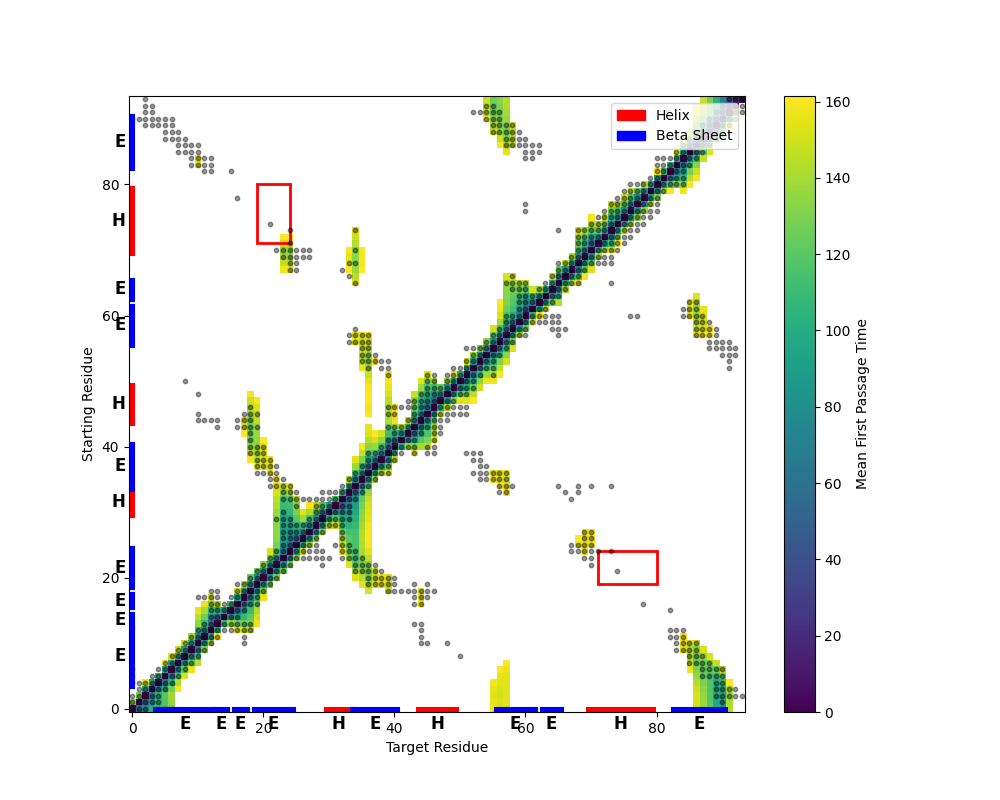
\includegraphics[width=0.8\textwidth]{/Users/enrico/PROTEINS/images/3LNX/first_time/Mean First Passage Time Matrix.png}
    \caption{Responses in time.}
\end{figure}

\begin{figure}[h!]
    \centering
    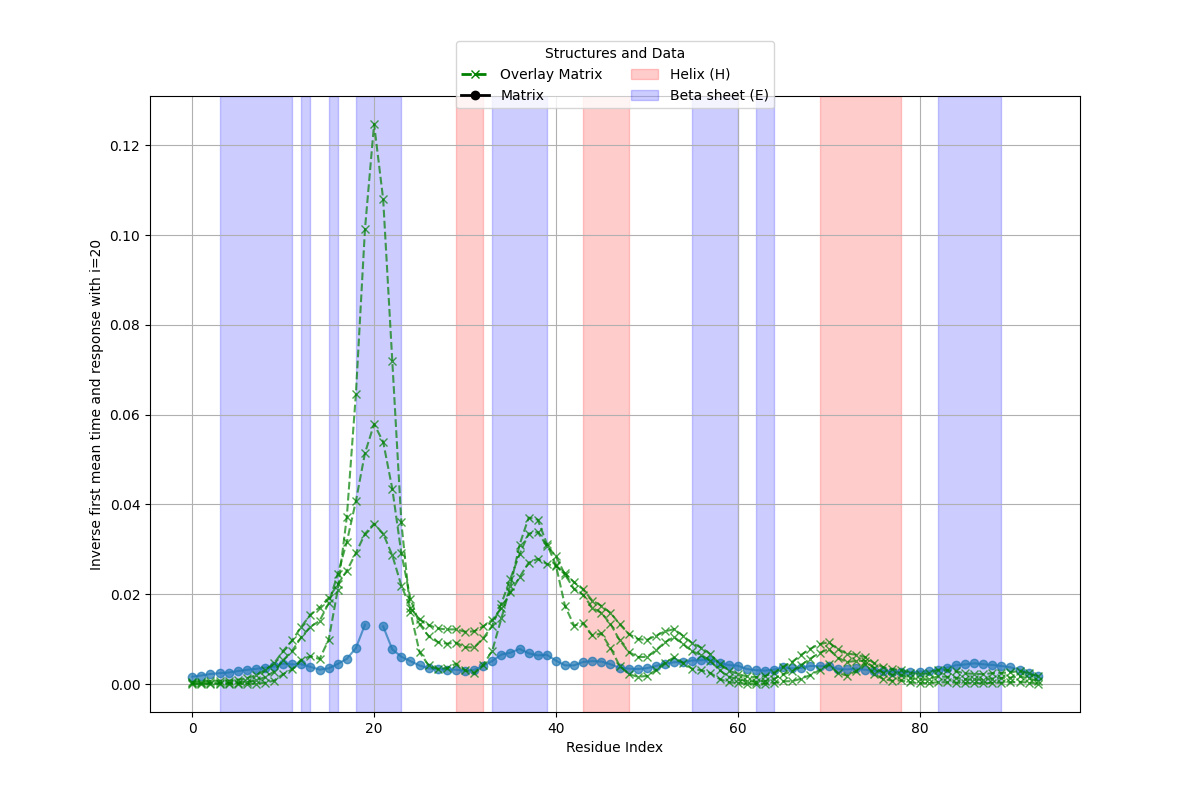
\includegraphics[width=0.8\textwidth]{/Users/enrico/PROTEINS/images/3LNX/Time_indicators/Inverse first mean time and response for i=20 as a function of j.png}
    \caption{Inverse first mean time perturbating 21-th residue.}
\end{figure}

\begin{figure}[h!]
    \centering
    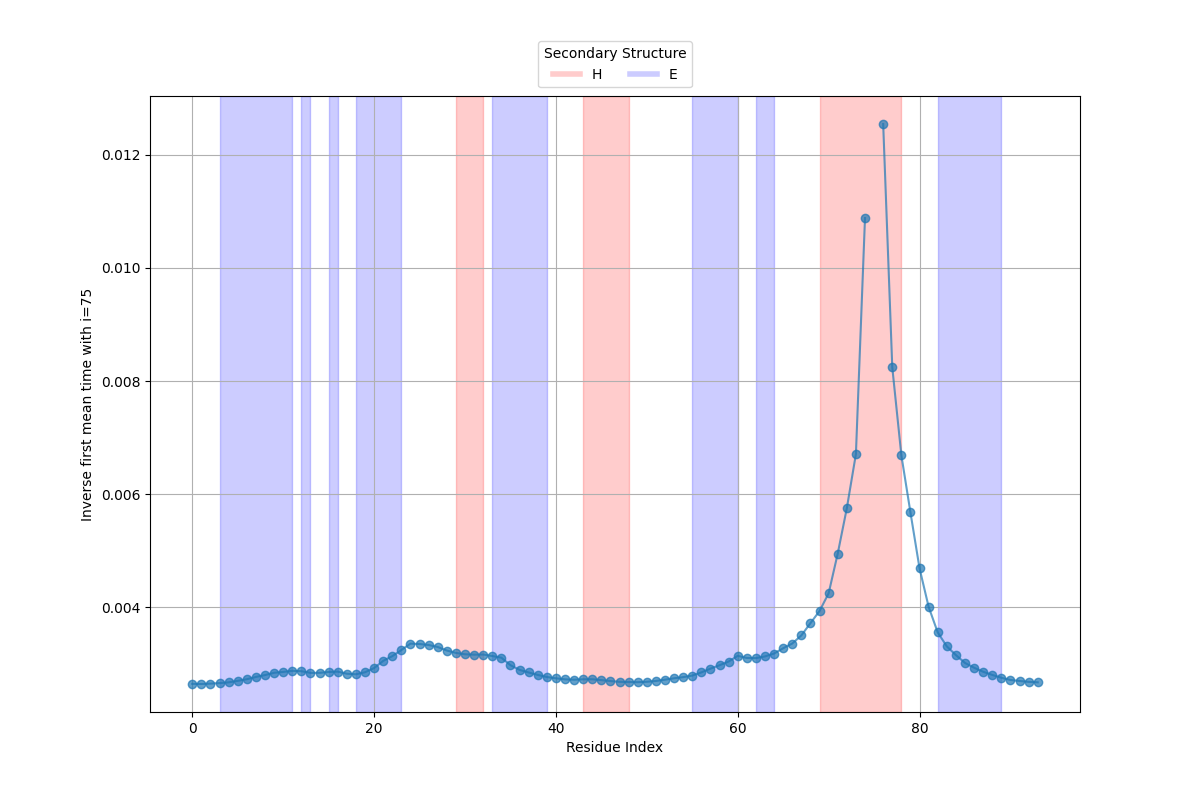
\includegraphics[width=0.8\textwidth]{/Users/enrico/PROTEINS/images/3LNX/Time_indicators/Inverse first mean time for i=75 as a function of j.png}
    \caption{Inverse first mean time perturbating 76-th residue.}
\end{figure}

\newpage
\newpage






\subsubsection*{Graphic Analysis of Secondary Structures}
The figures provide a detailed view of the dynamic properties of the protein structure, focusing on the beta sheet around residue ~20 and the alpha helix near residue ~75. These secondary structures exhibit distinct dynamical behaviors, which are quantified using metrics such as inverse first mean time, correlation, response, and transfer entropy.


\


\paragraph{Figure 6: Transfer Entropy with Residue ~20}
\begin{itemize}
    \item \textbf{Beta Sheet Region (Residue ~20):} High transfer entropy values in the beta sheet reflect strong localized information flow, emphasizing the beta sheet's role in stabilizing and coordinating motions within its region.
    \item \textbf{Alpha Helix Region (Residue ~75):} The helix shows lower transfer entropy values, indicating that it is less dynamically influenced by residue 20. This highlights the beta sheet's role as a local stabilizer rather than a global signal mediator.
    \item \textbf{Interpretation:} The beta sheet governs local dynamics through strong information flow, while the helix remains relatively decoupled in terms of direct influence.
\end{itemize}

\paragraph{Figure 7: Transfer Entropy with Residue ~75}
\begin{itemize}
    \item \textbf{Beta Sheet Region (Residue ~20):} Transfer entropy values indicate weak information flow from the helix to the beta sheet, consistent with the beta sheet's structural rigidity and localized dynamics.
    \item \textbf{Alpha Helix Region (Residue ~75):} Strong peaks in transfer entropy around residue 75 highlight its role in propagating dynamic information across the protein, making it a key mediator of long-range communication.
    \item \textbf{Interpretation:} The helix complements the beta sheet by actively facilitating dynamic interactions and communication throughout the protein.
\end{itemize}

\paragraph{Figure 8: Transfer Entropy Across Residues}
\begin{itemize}
    \item \textbf{Beta Sheet Region (Residue ~20):} The beta sheet demonstrates strong localized information transfer, confirming its role as a stabilizing region within the protein.
    \item \textbf{Alpha Helix Region (Residue ~75):} High transfer entropy values in the helix illustrate its central role in mediating long-range dynamic interactions, reinforcing its complementary function alongside the beta sheet.
    \item \textbf{Interpretation:} This figure synthesizes the overall dynamic behavior, showcasing the beta sheet as a stabilizing anchor and the helix as a mediator of dynamic adaptability and communication.
\end{itemize}
\newpage

\newpage
\null
\thispagestyle{empty}
\newpage
\begin{thebibliography}{100}

    \bibitem{ref} 
    \url{https://www.sciencelearn.org.nz/resources/209-role-of-proteins-in-the-body}
    
    \bibitem{ref2} 
    \emph{University of California Davis, Introductory Biology}, 
    \url{https://bio.libretexts.org/Courses/University_of_California_Davis/BIS_2A%3A_Introductory_Biology_%28Easlon%29/Readings/04.3%3A_Amino_Acids}
    
    \bibitem{ref3} 
    \emph{University of California Davis, Introductory Biology}, 
    \url{https://bio.libretexts.org/Courses/University_of_California_Davis/BIS_2A%3A_Introductory_Biology_%28Britt%29/01%3A_Readings/1.17%3A_Protein_Structure}
    
    \bibitem{ref4} 
    Nature, \url{https://www.nature.com/scitable/topicpage/protein-structure-14122136/}
    
    \bibitem{ref5} 
    Wikipedia, \url{https://en.wikipedia.org/wiki/Allosteric_regulation?utm_source=chatgpt.com}
    
    \bibitem{ref6} 
    Statistical Mechanics of Allosteric Enzymes
    
    \bibitem{ref7} 
    University of California Davis, Introductory Biology, Hemoglobin and allosteric effects
    
    \bibitem{ref8} 
    Allosterism in the PDZ Family, Amy O. Stevens and Yi He
    
    \bibitem{ref9} 
    Protein elastic network models and the ranges of cooperativity, Lei Yanga, Guang Songa, and Robert L. Jernigana
    
    \bibitem{ref11} 
    Introduzione alla Teoria dei Grafi, Vittorio Loreto, Francesca Tria.
    
    \bibitem{ref12} 
    Time- and ensemble-average statistical mechanics of the Gaussian network model, Alessio Lapolla, Maximilian Vossel, and Aljaz Godec
    
    \bibitem{ref13} 
    Correlation, response and entropy approaches to allosteric behaviors: a critical comparison on the ubiquitin case Fabio Cecconi, Giulio Costantini, Carlo Guardiani, Marco Baldovin and Angelo Vulpiani
    
    \bibitem{ref14} 
    Robust inference of causality in high-dimensional dynamical processes from the Information Imbalance of distance ranks
    Vittorio Del Tatto, Gianfranco Fortunato, Domenica Bueti, and Alessandro Laio
\end{thebibliography}

\end{document}